\documentclass{article}
\usepackage[backend=biber,natbib=true,style=alphabetic,maxbibnames=50]{biblatex}
\addbibresource{/home/nqbh/reference/bib.bib}
\usepackage[utf8]{vietnam}
\usepackage{tocloft}
\renewcommand{\cftsecleader}{\cftdotfill{\cftdotsep}}
\usepackage[colorlinks=true,linkcolor=blue,urlcolor=red,citecolor=magenta]{hyperref}
\usepackage{amsmath,amssymb,amsthm,enumitem,float,graphicx,mathtools,tikz}
\usetikzlibrary{angles,calc,intersections,matrix,patterns,quotes,shadings}
\allowdisplaybreaks
\newtheorem{assumption}{Assumption}
\newtheorem{baitoan}{}
\newtheorem{cauhoi}{Câu hỏi}
\newtheorem{conjecture}{Conjecture}
\newtheorem{corollary}{Corollary}
\newtheorem{dangtoan}{Dạng toán}
\newtheorem{definition}{Definition}
\newtheorem{dinhly}{Định lý}
\newtheorem{dinhnghia}{Định nghĩa}
\newtheorem{example}{Example}
\newtheorem{ghichu}{Ghi chú}
\newtheorem{hequa}{Hệ quả}
\newtheorem{hypothesis}{Hypothesis}
\newtheorem{lemma}{Lemma}
\newtheorem{luuy}{Lưu ý}
\newtheorem{nhanxet}{Nhận xét}
\newtheorem{notation}{Notation}
\newtheorem{note}{Note}
\newtheorem{principle}{Principle}
\newtheorem{problem}{Problem}
\newtheorem{proposition}{Proposition}
\newtheorem{question}{Question}
\newtheorem{remark}{Remark}
\newtheorem{theorem}{Theorem}
\newtheorem{vidu}{Ví dụ}
\usepackage[left=1cm,right=1cm,top=5mm,bottom=5mm,footskip=4mm]{geometry}
\def\labelitemii{$\circ$}
\DeclareRobustCommand{\divby}{%
	\mathrel{\vbox{\baselineskip.65ex\lineskiplimit0pt\hbox{.}\hbox{.}\hbox{.}}}%
}
\setlist[itemize]{leftmargin=*}
\setlist[enumerate]{leftmargin=*}

\title{Vietnamese Mathematical Olympiad for High School- {\it\&} College Students\\Olympic Toán Học Học Sinh {\it\&} Sinh Viên Toàn Quốc (VMC)}
\author{Nguyễn Quản Bá Hồng\footnote{A Scientist {\it\&} Creative Artist Wannabe. E-mail: {\tt nguyenquanbahong@gmail.com}. Bến Tre City, Việt Nam.}}
\date{\today}

\begin{document}
\maketitle
\begin{abstract}
	This text is a part of the series {\it Some Topics in Advanced STEM \& Beyond}:
	
	{\sc url}: \url{https://nqbh.github.io/advanced_STEM/}.
	
	Latest version:
	\begin{itemize}
		\item {\it Vietnamese Mathematical Olympiad for High School- \& College Students (VMC) -- Olympic Toán Học Học Sinh \& Sinh Viên Toàn Quốc}.
		
		PDF: {\sc url}: \url{https://github.com/NQBH/advanced_STEM_beyond/blob/main/VMC/NQBH_VMC.pdf}.
		
		\TeX: {\sc url}: \url{https://github.com/NQBH/advanced_STEM_beyond/blob/main/VMC/NQBH_VMC.tex}.
		\item Codes:
		\begin{itemize}
			\item C++ code: \url{https://github.com/NQBH/advanced_STEM_beyond/tree/main/VMC/C++}.
			\item Python code: \url{https://github.com/NQBH/advanced_STEM_beyond/tree/main/VMC/Python}.
		\end{itemize}
		\item Resource: \url{https://github.com/NQBH/advanced_STEM_beyond/tree/main/VMC/resource}.
		\item Figures: \url{https://github.com/NQBH/advanced_STEM_beyond/tree/main/VMC/figure}.
	\end{itemize}
\end{abstract}
\tableofcontents

%------------------------------------------------------------------------------%

\section*{Preliminaries -- Kiến thức chuẩn bị}

\textbf{\textsf{Resources -- Tài nguyên.}}
\begin{enumerate}
	\item \cite{Khai_so_hoc_day_so}. {\sc Phan Huy Khải}. {\it Các Chuyên Đề Số Học Bồi Dưỡng Học Sinh Giỏi Toán Trung Học. Chuyên Đề 2: Số Học \& Dãy Số}.
	\item {\sc VMS -- Hội Toán Học Việt Nam}. {\it Kỷ Yếu Kỳ Thi Olympic Toán Học Sinh Viên--Học Sinh Lần 28}.
	\item {\sc VMS -- Hội Toán Học Việt Nam}. {\it Kỷ Yếu Kỳ Thi Olympic Toán Học Sinh Viên--Học Sinh Lần 29}. Huế, 2--8.4.2023.
\end{enumerate}
Critical-thinking questions:
\begin{question}[Generalization; main ideas of a solution{\tt/}proof]
	What are main ideas of a solution or a proof of a problem that can be used to generalize the original problem?
\end{question}

\begin{question}[Link\footnote{Watch, e.g., \href{https://www.imdb.com/title/tt14976292/}{IMDb{\tt/}Shi Guang Dai Li Ren $\star$ Link Click} (2021--).}]
	Can we draw some link(s) between different problems? Even they are in different categories: algebra, analysis, \& combinatorics.
\end{question}

\subsection*{Notation -- Ký hiệu}

\begin{itemize}
	\item $\lfloor x\rfloor,\{x\}$ lần lượt được gọi là {\it phần nguyên \& phần lẻ} (integer- \& fractional parts) của $x\in\mathbb{R}$, see, e.g., \href{https://en.wikipedia.org/wiki/Floor_and_ceiling_functions}{Wikipedia{\tt/}floor \& ceiling functions}, \href{https://en.wikipedia.org/wiki/Fractional_part}{Wikipedia{\tt/}fractional part}.
	\item $x_+\coloneqq\max\{x,0\}$, $x_-\coloneqq\max\{-x,0\} = -\min\{x,0\}$ lần lượt được gọi là {\it phần dương \& phần âm} (positive- \& negative parts) của $x\in\mathbb{R}$.
\end{itemize}

%------------------------------------------------------------------------------%

\section{Algebra -- Đại Số}
\textbf{\textsf{Resources -- Tài nguyên.}}
\begin{enumerate}
	\item {\sc Bùi Xuân Hải, Trần Ngọc Hội, Trịnh Thanh Đèo, Lê Văn Luyện}. {\it Đại Số Tuyến Tính \& Ứng Dụng. Tập 1}. HCMUS.
	\item \cite{Hoa_linear_algebra}. {\sc Lê Tuấn Hoa}. {\it Đại Số Tuyến Tính Qua Các Ví Dụ \& Bài Tập}.
	\item \cite{Hung_linear_algebra}. {\sc Nguyễn Hữu Việt Hưng}. {\it Đại Số Tuyến Tính}. HNUS.
	\item \cite{Trefethen_Bau1997,Trefethen_Bau2022}. {\sc Lloyd N. Trefethen, David Bau III}. {\it Numerical Linear Algebra}.
	\item \cite{Trung_linear_algebra}. {\sc Ngô Việt Trung}. {\it Giáo Trình Đại Số Tuyến Tính}.
	\item \cite{Tsukada_Kobayashi_Kaneko_Takahasi_Shirayanagi_Noguchi2023}. {\sc Makoto Tsukada, Yuji Kobayashi, Hiroshi Kaneko, Sin-Ei Takahasi, Kiyoshi Shirayanagi, Masato Noguchi}. {\it Linear Algebra with Python: Theory \& Applications}.
\end{enumerate}

\begin{baitoan}[Symbolic computation software{\tt/}languages{\tt/}libraries for Linear Algebra]
	Tương tự như phần mềm {\sf MATLAB} \url{https://www.mathworks.com/products/matlab.html}, tìm các phần mềm, ngôn ngữ, hoặc thư viện của các ngôn ngữ quen thuộc như {\sf Python} (thư viện {\sf SymPy} \url{https://www.sympy.org/en/index.html}), {\sf C{\tt/}C++} để thực hành symbolic computation.
\end{baitoan}

%------------------------------------------------------------------------------%

\subsection{Matrix -- Ma trận}

\subsubsection{Determinant of a matrix -- Định thức của ma trận}
\begin{dinhnghia}
	{\rm Định thức} của 1 ma trận $A = (a_{ij})_{n\times n}$ với các yếu tố trong trường $\mathbb{F}$, được ký hiệu bởi $\det A$ hoặc $|A|$, là phần tử $\det A\coloneqq\sum_{\sigma\in S_n} {\rm sgn}(\sigma)a_{\sigma(1)1}\cdots a_{\sigma(n)n}$ của trường $\mathbb{F}$. Nếu $A$ là 1 ma trận vuông cỡ $n$ thì $\det A$ được gọi là 1 {\rm định thức cỡ $n$}. Tổng ở vế phải của đẳng thức này có tất cả $|S_n| = n!$ số hạng.
\end{dinhnghia}

\begin{vidu}
	(a) Định thức cỡ 1: $\det(a) = a$, $\forall a\in\mathbb{F}$. (b) Định thức cỡ 2:
	\begin{equation*}
		\det\begin{pmatrix}
			a_{11} & a_{12}\\a_{21} & a_{22}
		\end{pmatrix} = \begin{vmatrix}
			a_{11} & a_{12}\\a_{21} & a_{22}
		\end{vmatrix} = a_{11}a_{22} - a_{21}a_{12}.
	\end{equation*}
	(c) Định thức cỡ 3:
	\begin{equation*}
		\det\begin{pmatrix}
			a_{11} & a_{12} & a_{13}\\a_{21} & a_{22} & a_{23}\\a_{31} & a_{32} & a_{33}
		\end{pmatrix} = \begin{vmatrix}
			a_{11} & a_{12} & a_{13}\\a_{21} & a_{22} & a_{23}\\a_{31} & a_{32} & a_{33}
		\end{vmatrix} = a_{11}a_{22}a_{33} + a_{21}a_{32}a_{13} + a_{31}a_{12}a_{23} - a_{11}a_{32}a_{23} - a_{21}a_{12}a_{33} - a_{31}a_{22}a_{13}.
	\end{equation*}
\end{vidu}
Trên thực tế, không trực tiếp dùng định nghĩa để tính các định thức cỡ $n > 3$ vì việc này quá phức tạp.

Gọi ${\bf a}_j\in\mathbb{F}^n$ là vector cột thứ $j$ của ma trận $A$, \& coi $\det A$ là 1 hàm của $n$ vector ${\bf a}_1,\ldots,{\bf a}_n$. Viết $\det A = \det({\bf a}_1,\ldots,{\bf a}_n)$.

\begin{dinhly}[3 tính chất cơ bản của định thức]
	(i) {\rm(Multilinear -- Đa tuyến tính)} Định thức của ma trận là 1 hàm tuyến tính với mỗi cột (resp., hàng) của nó, khi cố định các cột (resp., hàng) khác, i.e.:
	\begin{equation*}
		\det({\bf a}_1,\ldots,a{\bf a}_j + b{\bf b}_j,\ldots,{\bf a}_n) = a\det({\bf a}_1,\ldots,{\bf a}_j,\ldots,{\bf a}_n) + b\det({\bf a}_1,\ldots,{\bf b}_j,\ldots,{\bf a}_n),\ \forall a,b\in\mathbb{F},\ {\bf a}_1,\ldots,{\bf a}_j,{\bf b}_j,\ldots,{\bf a}_n\in\mathbb{F}^n,\ j = 1,\ldots,n.
	\end{equation*}
	(ii) {\rm(Thay phiên)} Nếu ma trận vuông $A$ có 2 cột (resp., hàng) bằng nhau thì $\det A = 0$. (iii) {\rm(Chuẩn hóa)} Định thức của ma trận đơn vị bằng $1$: $\det I_n = 1$. (iv) Định thức là hàm duy nhất trên các ma trận vuông có 3 tính chất (i)--(iii).
\end{dinhly}

\begin{hequa}[\cite{Hung_linear_algebra}, Hệ quả 2.3, p. 137]
	(i) {\rm(Tính phản đối xứng của định thức)} Nếu đổi chỗ 2 cột (resp., hàng) của 1 ma trận thì định thức của nó đổi dấu:
	\begin{equation*}
		\det(\ldots,{\bf a}_i,\ldots,{\bf a}_j,\ldots) = -\det(\ldots,{\bf a}_j,\ldots,{\bf a}_i,\ldots).
	\end{equation*}
	(ii) Nếu các vector cột (resp., vector hàng) của 1 ma trận phụ thuộc tuyến tính thì định thức của ma trận bằng $0$. Nói riêng, nếu ma trận có 1 cột (resp., hàng) bằng $0$ thì định thức của nó bằng $0$. (iii) Nếu thêm vào 1 cột (resp., hàng) của ma trận 1 tổ hợp tuyến tính của các cột (resp., hàng) khác thì định thức của nó không thay đổi.
\end{hequa}
Các tính chất của định thức đối với các hàng cũng tương tự các tính chất của định thức đối với các cột. 1 phương pháp tính định thúc có hiệu quả là ứng dụng các tính chất đó để biến đổi ma trận thành 1 ma trận tam giác có cùng định thức.

\begin{dinhnghia}[Ma trận tam giác]
	Ma trận $A$ được gọi là 1 {\rm ma trận tam giác trên} nếu nó có dạng
	\begin{equation*}
		A = \begin{pmatrix}
			a_{11} & a_{12} & \cdots & a_{1n}\\0 & a_{22} & \cdots & a_{2n}\\
			\vdots & \vdots & \ddots & \vdots\\0 & 0 & \cdots & a_{nn}
		\end{pmatrix},
	\end{equation*}
	trong đó $a_{ij} = 0$ với $i > j$. Tương tự, $A$ được gọi là 1 {\rm ma trận tam giác dưới} nếu $a_{ij} = 0$ với $i < j$. Ma trận tam giác trên \& ma trận tam giác dưới được gọi chung là {\rm ma trận tam giác}.
\end{dinhnghia}

\begin{dinhly}[Định thức của ma trận tam giác]
	Nếu $A$ là 1 ma trận tam giác cỡ $n$ thì $\det A = \prod_{i=1}^n a_{ii} = a_{11}a_{22}\cdots a_{nn}$.
\end{dinhly}

\begin{dinhly}[\cite{Hung_linear_algebra}, Định lý 5.1, p. 147]
	Giả sử $A,B\in M(n\times n,\mathbb{F})$. Khi đó: (i) $\det(AB) = \det A\det B$. (ii) $A$ khả nghịch $\Leftrightarrow\det A\ne0$. Hơn nữa, $\det(A^{-1}) = (\det A)^{-1} = \frac{1}{\det A}$, hay $\det A\det(A^{-1}) = 1$. (iii) Định thức của ma trận chuyển vị: $\det(A^\top) = \det A$, $\forall A\in M(n\times n,\mathbb{F})$.
\end{dinhly}
Theo định lý này, tất cả các tính chất của định thức đối với các cột của nó vẫn đúng đối với các hàng của nó. E.g., định thức là 1 hàm đa tuyến tính, thay phiên, \& chuẩn hóa đối với các hàng của nó, $\ldots$

\begin{baitoan}[Tính $\det A$ bằng cách hạ cấp]
	Tính định thức cỡ $n$ thông qua các định thức nhỏ hơn.
\end{baitoan}
Cho $A = (a_{ij})\in M(n\times n,\mathbb{F})$ \& $k\in\mathbb{N}$ thỏa $1\le k < n$. Xét 2 bộ chỉ số $1\le i_1 < i_2 < \cdots < i_k\le n$, $1\le j_1 < j_2 < \cdots < j_k\le n$. Các phần tử nằm trên giao của $k$ hàng $i_1,\ldots,i_k$ \& $k$ cột $j_1,\ldots,j_k$ của ma trận $A$ lập nên 1 ma trận cỡ $k$, được gọi là 1 {\it ma trận con cỡ $k$} của $A$, \& định thức của ma trận con đó, được ký hiệu là $D_{i_1,\ldots,i_k}^{j_1,\ldots,j_k}$, được gọi là 1 {\it định thức con cỡ $k$} của $A$.

Nếu xóa tất cả các hàng $i_1,\ldots,i_k$ \& các cột $j_1,\ldots,j_k$ thì phần còn lại của ma trận $A$ lập nên 1 ma trận vuông cỡ $n - k$, mà định thức của nó được ký hiệu là $\overline{D}_{i_1,\ldots,i_k}^{j_1,\ldots,j_k}$ \& được gọi là {\it định t hức con bù} của $D_{i_1,\ldots,i_k}^{j_1,\ldots,j_k}$. Gọi $(-1)^{s(I,J)}\overline{D}_{i_1,\ldots,i_k}^{j_1,\ldots,j_k}$ là {\it phần bù đại số} của $D_{i_1,\ldots,i_k}^{j_1,\ldots,j_k}$ (trong định thức của $A$), với $s(I,J)\coloneqq\sum_{n=1}^k i_n + j_n = (i_1 + \cdots + i_k) + (j_1 + \cdots + j_k)$.

\begin{dinhly}[Khai triển Laplace, \cite{Hung_linear_algebra}, Định lý 5.3, pp. 148--149]
	Giả sử đã chọn ra $k$ cột (resp., $k$ hàng) trong 1 định thức cỡ $n$ ($1\le k < n$). Khi đó, định thức đã cho bằng tổng của tất cả các tích của các định thức con cỡ $k$ lấy ra từ $k$ cột (resp., $k$ hàng) đã chọn với phần bù đại số của chúng. Nói rõ hơn: (i) Công thức khai triển định thức theo $k$ cột $j_1 < \cdots < j_k$:
	\begin{equation*}
		\det A = \sum_{i_1 < \cdots < i_k} (-1)^{(s(I,J))}D_{i_1,\ldots,i_k}^{j_1,\ldots,j_k}\overline{D}_{i_1,\ldots,i_k}^{j_1,\ldots,j_k}.
	\end{equation*}
	(ii) Công thức khai triển định thức theo $k$ hàng $i_1 < \cdots < i_k$:
	\begin{equation*}
		\det A = \sum_{j_1 < \cdots < j_k} (-1)^{(s(I,J))}D_{i_1,\ldots,i_k}^{j_1,\ldots,j_k}\overline{D}_{i_1,\ldots,i_k}^{j_1,\ldots,j_k}.
	\end{equation*}
\end{dinhly}

\begin{baitoan}[Định thức Vandermonde]
	Tính định thức Vandermonde
	\begin{equation*}
		D_n\coloneqq\begin{vmatrix}
			1 & x_1 & x_1^2 & \cdots & x_1^{n-1}\\
			1 & x_2 & x_2^2 & \cdots & x_2^{n-1}\\
			\vdots & \vdots & \vdots & \ddots & \vdots\\
			1 & x_n & x_n^2 & \cdots & x_n^{n-1}\\
		\end{vmatrix}.
	\end{equation*}
\end{baitoan}
{\sf Hint.} Làm cho hầu hết các phần tử của hàng cuối của $D_n$ trở thành 0 bằng cách lấy cột thứ $n - 1$ nhân với $-x_n$ rồi cột vào cột $n$, rồi lấy cột thứ $n - 2$ nhân với $-x_n$ rồi cộng vào cột $n - 1$, $\ldots$, cuối cùng lấy cột thứ nhất nhân với $-x_n$ rồi cộng vào cột 2, i.e., ${\bf c}_i = {\bf c}_i + (-x_n){\bf c}_{i-1} = {\bf c}_i - x_n{\bf c}_{i-1}$ với $i = n,n - 1,\ldots,2$ (chạy lui). Khai triển Laplace theo hàng thứ $n$, đưa các thừa số chung của mỗi hàng ra ngoài dấu định thức, được công thức truy toán{\tt/}hồi: $D_n = (x_n - x_1)(x_n - x_2)\cdots(x_n - x_{n-1})D_{n-1} = \prod_{i=1}^{n-1} (x_n - x_i)D_{n-1}$. Quy nạp với $D_1 = 1$ được
\begin{equation}
	\label{Vandermonde det}
	\tag{Vandermonde}
	D_n = \prod_{1\le j < i\le n} (x_i - x_j),\ \forall n\in\mathbb{N}^\star.
\end{equation}
1 ứng dụng quan trọng của khai triển Laplace là công thức tính ma trận nghịch đảo:

\begin{dinhly}[Công thức tính ma trận nghịch đảo, \cite{Hung_linear_algebra}, Định lý 5.4, p. 152]
	(i) Nếu ma trận vuông $A = (a_{ij})\in M(n\times n,\mathbb{F})$ có định thức khác $0$ thì $A$ khả nghịch \&
	\begin{equation*}
		A^{-1} = \frac{1}{\det A}\begin{pmatrix}
			\tilde{a}_{11} & \cdots & \tilde{a}_{n1}\\\vdots & \ddots & \vdots\\\tilde{a}_{1n} & \cdots & \tilde{a}_{nn}
		\end{pmatrix},
	\end{equation*}
	với $\tilde{a}_{ij}$ là phần bù đại số của $a_{ij}$ trong định thức của $A$. (ii) {\rm Ma trận phụ hợp} (adjugate matrix) của $A$ được định nghĩa bởi:
	\begin{equation*}
		{\rm adj}(A) = \begin{pmatrix}
			\tilde{a}_{11} & \cdots & \tilde{a}_{n1}\\\vdots & \ddots & \vdots\\\tilde{a}_{1n} & \cdots & \tilde{a}_{nn}
		\end{pmatrix},
	\end{equation*}
	thì $A{\rm adj}(A) = {\rm adj}(A)A = \det A I_n$, (i) viết lại thành $A^{-1} = \frac{1}{\det A}{\rm adj}(A)$.
\end{dinhly}
For more properties of adjugate matrix, see, e.g., \href{https://en.wikipedia.org/wiki/Adjugate_matrix}{Wikipedia{\tt/}adjugate matrix}.

%------------------------------------------------------------------------------%

\subsubsection{Rank of a matrix -- Hạng của ma trận}
Hạng của 1 ma trận là hạng của hệ vector cột (hoặc hệ vector hàng) của nó. Định lý sau cho phép tính hạng của ma trận thông qua định thức:

\begin{dinhly}[Công thức tính hạng của ma trận, \cite{Hung_linear_algebra}, Định lý 6.1, p. 153, Hệ quả 6.2, p. 154]
	(i) Giả sử $A$ là 1 ma trận $m$ hàng $n$ cột, với các yếu tố trong trường $\mathbb{F}$. Khi đó, hạng của ma trận $A$ bằng cỡ lớn nhất của các định thức con khác $0$ của $A$. Nói rõ hơn, $\operatorname{rank}A = r$ nếu có 1 định thức con cỡ $r$ của $A$ khác $0$, \& mọi định thức con cỡ $> r$ (nếu có) của $A$ đều bằng $0$. (ii) Hạng của 1 ma trận bằng hạng của hệ các vector hàng của nó.
\end{dinhly}
{\it Quan hệ giữa định thức \& hạng}:
\begin{equation*}
	\forall A\in M(\mathbb{F},n\times n),\ \det A\ne0\Leftrightarrow\operatorname{rank}A = n,\ \det A = 0\Leftrightarrow\operatorname{rank}A < n.
\end{equation*}

%------------------------------------------------------------------------------%

\subsubsection{System of linear equations \& Cramer rule -- Hệ phương trình tuyến tính \& quy tắc Cramer}

\begin{dinhnghia}
	1 hệ thống có dạng
	\begin{equation}
		\label{linear system: explicit form}
		\left\{\begin{split}
			a_{11}x_1 + a_{12}x_2 + \cdots + a_{1n}x_n &= b_1,\\
			a_{21}x_1 + a_{22}x_2 + \cdots + a_{2n}x_n &= b_2,\\
			&\cdots\\
			a_{m1}x_1 + a_{m2}x_2 + \cdots + a_{mn}x_n &= b_m,\\
		\end{split}\right.
	\end{equation}
	trong đó $a_{ij},b_i\in\mathbb{F}$ là các phần tử cho trước, được gọi là 1 {\rm hệ phương trình tuyến tính} gồm $m\in\mathbb{N}^\star$ phương trình với $n\in\mathbb{N}^\star$ ẩn $x_1,\ldots,x_n$. Ký hiệu
	\begin{equation*}
		A = (a_{ij})_{m\times n},\ {\bf x} = \begin{pmatrix}
			x_1\\\vdots\\x_n
		\end{pmatrix},\ {\bf b} = \begin{pmatrix}
			b_1\\\vdots\\b_m
		\end{pmatrix}.
	\end{equation*}
	Khi đó, hệ phương trình \eqref{linear system: explicit form} có thể được viết dưới dạng phương trình vector:
	\begin{equation}
		\label{linear system: vector form}
		A{\bf x} = {\bf b}.
	\end{equation}
	1 {\rm nghiệm} của hệ này là 1 vector ${\bf x}^0\in\mathbb{F}^n$ để $A{\bf x}^0 = {\bf b}$. 1 hệ phương trình có ít nhất 1 nghiệm được gọi là 1 {\rm hệ phương trình tương thích}. Hệ phương trình $A{\bf x} = {\bf0}$ được gọi là {\rm hệ phương trình tuyến tính thuần nhất} liên kết với hệ $A{\bf x} = {\bf b}$.
\end{dinhnghia}
Cảm nhận: Hệ phương trình tuyến tính \eqref{linear system: vector form} có nghiệm duy nhất nếu số phương trình của hệ bằng số ẩn, \& không có phương trình nào của hệ là ``hệ quả'' của các phương trình khác (i.e., tổ hợp tuyến tính của các phương trình khác).

\begin{dinhnghia}[Hệ không suy biến{\tt/}Cramer, \cite{Hung_linear_algebra}, Định nghĩa 7.1, p. 156]
	Hệ phương trình tuyến tính \eqref{linear system: vector form} được gọi là 1 {\rm hệ không suy biến} (hay 1 {\rm hệ Cramer}) nếu nó có số phương trình bằng số ẩn (i.e., nếu $A$ là 1 ma trận vuông) \& nếu $\det A\ne 0$.
\end{dinhnghia}

\begin{dinhly}[Tính giải được duy nhất của hệ Cramer, \cite{Hung_linear_algebra}, Định lý 7.2, p. 156]
	Hệ phương trình tuyến tính không suy biến \eqref{linear system: vector form} có 1 nghiệm duy nhất, được tính bằng công thức
	\begin{equation*}
		x_j = \frac{\det A_j}{\det A},\ j = 1,\ldots,n,
	\end{equation*}
	với $A_j$ là ma trận nhận được từ ma trận $A$ bằng cách thay cột thứ $j$ bởi cột hệ số tự do ${\bf b}$.
\end{dinhly}

%------------------------------------------------------------------------------%

\subsubsection{System of linear equations \& Gauss elimination method -- Hệ phương trình tuyến tính \& phương pháp khử Gauss}
Phương pháp Cramer chỉ áp dụng cho được (range of applicability) cho các hệ phương trình tuyến tính không suy biến (nói riêng, các hệ này có số phương trình bằng số ẩn) (why? vì nếu hệ suy biến, tức hoặc ma trận $A$ không vuông, khi đó $\det A$ không có nghĩa, hoặc $\det A = 0$, khi đó công thức nghiệm cho bởi quy tắc Cramer không xác định vì mẫu số bằng 0). Nhưng rất nhiề hệ phương trình tuyến tính ta gặp, đặc biệt là trong thực tế, lại suy biến. Phương pháp khử Gauss (Gauss elimination method) có ưu điểm là có thể áp dụng cho hệ phương trình tuyến tính tùy ý. Nhược điểm của phương pháp khử Gauss là không đưa ra đuọc thông tin nào về nghiệm của hệ phương trình trước khi giải xong hệ đó.

Về mặt trực giác, phương pháp Cramer mang tính chất toán học để xác định được cấu trúc nghiệm của hệ phương trình tuyến tính không suy biến hơn, còn phương pháp khử Gauss mang tính chất của 1 thuật toán, 1 quy trình hơn là 1 phương pháp toán dùng để xác định cấu trúc nghiệm của hệ phương trình tuyến tính.

\begin{dinhnghia}
	2 hệ phương trình được gọi là {\rm tương đương} nếu nghiệm của hệ này cũng là nghiệm của hệ kia \& ngược lại, i.e., 2 hệ phương trình có cùng tập nghiệm.
\end{dinhnghia}

\begin{dinhly}[3 phép biến đổi sơ cấp]
	Nếu ta áp dụng các phép biến đổi sau:
	\item(i) Đổi chỗ 2 phương trình của hệ.
	\item(ii) Nhân 1 phương trình của hệ với 1 vô hướng khác $0$ thuộc trường $\mathbb{F}$.
	\item(iii) Cộng vào 1 phương trình 1 tổ hợp tuyến tính của các phương trình khác trong hệ.
	
	((i)--(iii) được gọi là các {\rm phép biến đổi sơ cấp}), trên 1 hệ phương trình tuyến tính, thì ta nhận được 1 hệ phương trình tuyến tính tương đương với hệ ban đầu.
\end{dinhly}
Xét 1 hệ phương trình tuyến tính tổng quát \eqref{linear system: explicit form}. Gọi $A = (a_{ij})_{m\times n}$ là {\it ma trận các hệ số} \&
\begin{equation*}
	\overline{A} = \begin{pmatrix}
		a_{11} & a_{12} & \cdots & a_{1n} & b_1\\
		a_{21} & a_{22} & \cdots & a_{2n} & b_2\\
		\vdots & \vdots & \ddots & \vdots & \cdot\\
		a_{m1} & a_{m2} & \cdots & a_{mn} & b_m
	\end{pmatrix}
\end{equation*}
là {\it ma trận các hệ số mở rộng} của hệ phương trình \eqref{linear system: explicit form}. Giả sử có 1 hê số nào đó $a_{ij}\ne0$. W.l.o.g. (nếu cần, đổi chỗ các phương trình \& đánh số lại các ẩn) có thể coi $a_{11}\ne0$. Khi đó, nhân phương trình thứ nhất với $-\frac{a_{i1}}{a_{11}}$ rồi cộng vào phương trình thứ $i$ ($i = 2,\ldots,m$), nhận được hệ phương trình tương đương. Lặp lại lập luận trên đối với hệ còn gồm $n - 1$ phương trình cuối với các ẩn $x_2,\ldots,x_n$. Sau 1 số bước hữu hạn, nhận được 1 hệ tương đương với ma trận mở rộng có dạng $(\overline{A}|\overline{b})$ với $\overline{A}$ là 1 ma trận dạng bậc thang.

Tương ứng với các phép biến đổi sơ cấp trên hệ phương trình tuyến tính là các phép {\it biến đổi sơ cấp} trên ma trận:
\begin{enumerate}
	\item Đổi chỗ 2 hàng (hoặc 2 cột) của ma trận.
	\item Nhân 1 hàng (hoặc 1 cột) của ma trận với 1 vô hướng khác $0$.
	\item Cộng vào 1 hàng (hoặc 1 cột) 1 tổ hợp tuyến tính của các hàng (resp., các cột) khác.
\end{enumerate}
Vì các phép biến đổi sơ cấp không làm thay đổi hạng của ma trận (why?) nên dẫn tới 1 cách tính hạng của ma trận giàu tính thực hành: Mỗi ma trận $A = (a_{ij})_{m\times n}$ sau 1 số hữu hạn phép biến đổi sơ cấp đều có thể đưa về 1 ma trận dạng tam giác trên, số dòng có chứa phần tử $\ne0$ bằng $\operatorname{rank}A$.

\begin{remark}[Ứng dụng của phương pháp khử Gauss để tìm ma trận nghịch đảo]
	Để tìm nghịch đảo (nếu có) của ma trận $A = (a_{ij})_{n\times n}$, lập ma trận $n\times2n$: $(A,I_n)$. Dùng 2 loại phép biến đổi hàng:
	\item(r1) Nhân 1 hàng với 1 vô hướng khác $0$,
	\item(r2) Cộng vào 1 hàng 1 tổ hợp tuyến tính của các hàng khác,
	
	\noindent để đưa ma trận $(A,I_n)$ về dạng $(I_n,B)$. Khi đó, $B = A^{-1}$. Ma trận $A$ không có nghịch đảo $\Leftrightarrow$ ma trận $(A,I_n)$ không thể đưa về ma trận dạng $(I_n,B)$ bằng 2 loại phép biến đổi hàng (r1) \& (r2).
\end{remark}

%------------------------------------------------------------------------------%

\subsubsection{Cấu trúc nghiệm của hệ phương trình tuyến tính}
See, e.g., \cite[Chap. 3, \S9: Cấu trúc nghiệm của hệ phương trình tuyến tính, pp. 163--165]{Hung_linear_algebra}.

Xét các hệ phương trình tuyến tính thuần nhất \& không thuần nhất liên kết với nhau $A{\bf x} = {\bf0}$ \& $A{\bf x} = {\bf b}$ \eqref{linear system: vector form}, với $A = (a_{ij})_{m\times n}\in M(m\times n,\mathbb{F}),{\bf b}\in\mathbb{F}^m$ (cả 2 hệ phương trình đều gồm $m$ phương trình \& $n$ ẩn).

\begin{dinhly}[\cite{Hung_linear_algebra}, Định lý 9.1, p. 163]
	Tập hợp $L$ tất cả các nghiệm của hệ phương trình tuyến tính thuần nhất $Ax = 0$ là 1 không gian vector con của $\mathbb{F}^n$, có số chiều thỏa mãn hệ thức $\dim L = n - \operatorname{rank}A$.
\end{dinhly}
$L\coloneqq\operatorname{Ker}\tilde{A}$ với $\tilde{A}:\mathbb{F}^n\to\mathbb{F}^m$, ${\bf x}\mapsto A{\bf x}$, i.e., $L$ là hạt nhân{\tt/}hạch của ánh xạ tuyến tính $\tilde{A}$.

\begin{dinhly}[\cite{Hung_linear_algebra}, Định lý 9.2, p. 164]
	Giả sử $L$ là không gian vector con gồm các nghiệm của hệ phương trình tuyến tính thuần nhất $A{\bf x} = {\bf0}$, \& ${\bf x}^0$ là 1 nghiệm của hệ $A{\bf x} = {\bf b}$. Khi đó tập hợp các nghiệm của hệ $A{\bf x} = {\bf b}$ là ${\bf x}^0 + L = \{{\bf x}^0 + {\bf a}|{\bf a}\in L\}$.
\end{dinhly}

\begin{dinhnghia}[Nghiệm riêng \& nghiệm tổng quát của hệ phương trình tuyến tính không thuần nhất]
	Với các giả thiết của định lý trên, ${\bf x}^0$ được gọi là 1 \emph{nghiệm riêng} của hệ phương trình tuyến tính không thuần nhất $A{\bf x} = {\bf b}$. Còn ${\bf x}^0 + {\bf a}$ với ${\bf a}\in L$, được gọi là \emph{nghiệm tổng quát} của hệ phương trình đó.
\end{dinhnghia}

\begin{dinhly}[\cite{Hung_linear_algebra}, Định lý 9.4: Tiêu chuẩn Kronecker--Capelli, p. 164]
	Hệ phương trình tuyến tính $A{\bf x} = {\bf b}$ có nghiệm $\Leftrightarrow\operatorname{rank}A = \operatorname{rank}\overline{A}$ với $\overline{A} = (A|{\bf b})$ là ma trận các hệ số mở rộng của hệ.
\end{dinhly}

\begin{baitoan}[VMC2023B1]
	(a) Cho $x\in\mathbb{R}$. Tính $\det A$ theo $x$ với
	\begin{equation*}
		A = \begin{pmatrix}
			x & 2022 & 2023\\2022 & 2023 & x\\2023 & x & 2022
		\end{pmatrix}.
	\end{equation*}
	(b) Tìm $x\in\mathbb{R}$ để $\operatorname{rank}A < 3$. Tính $\operatorname{rank}A$ với $x$ vừa tìm được.
\end{baitoan}
{\sf Hint.} Tổng mỗi dòng \& mỗi cột của ma trận $A$ đều bằng $x + 2022 + 2023$.

\begin{proof}[Giải]
	(a) Đặt $a\coloneqq2022$. Cộng hàng 2 \& hàng 3 vào hàng 1 được:
	\begin{align*}
		&\begin{vmatrix}
			x & a & a + 1\\a & a + 1 & x\\a + 1 & x & a
		\end{vmatrix} = (x + 2a + 1)\begin{vmatrix}
			1 & 1 & 1\\a & a + 1 & x\\a + 1 & x & a
		\end{vmatrix} = (x + 2a + 1)\begin{vmatrix}
			1 & 0 & 0\\a & 1 & x - a\\a + 1 & x - a - 1 & -1
		\end{vmatrix} = (x + 2a + 1)\begin{vmatrix}
			1 & x - a\\x - a - 1 & -1
		\end{vmatrix}\\
		&= (x + 2a + 1)[-1 - (x - a)(x - a - 1)] = -(x + 2a + 1)(x^2 - (2a + 1)x + a^2 + a + 1) = -(x + 4045)(x^2 - 4045x + 4090507).
	\end{align*}
	(b) $\operatorname{rank}A < 3\Leftrightarrow\det A = 0\Leftrightarrow(x + 4045)(x^2 - 4045x + 4090507)\Leftrightarrow x = -4045$ vì $\Delta = (2a + 1)^2 - 4(a^2 + a + 1) = -3 < 0$ nên vô nghiệm thực. Khi $x = -4045$, $\operatorname{rank}A$ bằng hạng của ma trận
	\begin{equation*}
		\begin{pmatrix}
			0 & 0 & 0\\2022 & 2023 & -4045\\2023 & -4045 & 2022
		\end{pmatrix}
	\end{equation*}
	Vậy $\operatorname{rank}A = 2$ khi $x = -4045$.
\end{proof}

\begin{nhanxet}
	(i) Việc đặt $a\coloneqq2022$ giúp thấy được cấu trúc chung của ma trận, không bị ảnh hưởng bởi các tính toán số cụ thể, đặc biêt giúp đơn giản hóa việc tính biệt thức $\Delta$ để chứng minh nhân tử phương trình bậc 2 trong $\det A$ vô nghiệm thực. (ii) Có thể tính $\det A$ bằng thư viện {\tt SymPy} của Python bằng cách chạy:
	\begin{verbatim}
		from sympy.matrices import Matrix, eye, zeros, ones, diag, GramSchmidt
		from sympy import factor
		
		# VMC2023B1
		from sympy.abc import x, a
		A = Matrix([[x, a, a + 1], [a, a + 1, x], [a + 1, x, a]])
		detA = A.det()
		print(detA)
		print(factor(detA))
	\end{verbatim}
	để thu được:
	\begin{verbatim}
		-2*a**3 + 3*a**2*x - 3*a**2 + 3*a*x - 3*a - x**3 - 1
		-(2*a + x + 1)*(a**2 - 2*a*x + a + x**2 - x + 1)
	\end{verbatim}
	i.e., $\det A = -(x + 2a + 1)(x^2 - (2a + 1)x + a^2 + a + 1)$ như đã tính.
\end{nhanxet}

\begin{baitoan}[VMC2023B2]
	Giả sử $f:\mathbb{R}^4\to\mathbb{R}^3$ là ánh xạ tuyến tính cho bởi:
	\begin{equation*}
		(x_1,x_2,x_3,x_4)\mapsto(x_1 + \lambda x_2 - x_3 + 2x_4,2x_1 - x_2 + \lambda x_3 + 5x_4,x_1 + 10x_2 - 6x_3 + x_4),
	\end{equation*}
	với $\lambda\in\mathbb{R}$: tham số. (a) Với $\lambda = 3$, tìm: (a1) 1 cơ sở \& số chiều của không gian hạt nhân $\operatorname{Ker}$. (a2) 1 cơ sở \& số chiều của không gian ảnh ${\rm Im}(f)$. (b) Tìm $\dim\operatorname{Im}f$ theo $\lambda$.
\end{baitoan}

\begin{proof}[Giải]
	Ánh xạ tuyến tính $f$ có ma trận trong cặp cơ sở chính tắc của $\mathbb{R}^4$ \& $\mathbb{R}^3$ là:
	\begin{equation*}
		A(\lambda) = \begin{pmatrix}
			1 & \lambda & -1 & 2\\2 & -1 & \lambda & 5\\1 & 10 & -6 & 1
		\end{pmatrix}
	\end{equation*}
	(a) Với $\lambda = 3$, hạt nhân $\operatorname{Ker}f$ là không gian nghiệm của phương trình thuần nhất với ma trận hệ số:
	\begin{equation*}
		A(3) = \begin{pmatrix}
			1 & 3 & -1 & 2\\2 & -1 & 3 & 5\\1 & 10 & -6 & 1
		\end{pmatrix},
	\end{equation*}
	Dùng phép biến đổi sơ cấp trên dùng suy ra $\dim\operatorname{Ker}f = 2$ với 1 cơ sở $(-8,5,7,0),(-17,1,0,7)$. Suy ra $\dim\operatorname{Im}f = n - \dim\operatorname{Ker}f = 4 - 2 = 2$. Vì mỗi vector thuộc $\operatorname{Im}f$ là 1 tổ hợp tuyến tính của các vector cột của $A(3)$ nên ảnh của ánh xạ $f$ là không gian cong sinh bởi các vector cột. Dùng các phép biến đổi sơ cấp trên dòng cho $A^\top$ suy ra 1 cơ sở của $operatorname{Im}f$ là $(1,2,1),(0,1,-1)$. (b) $ \dim\operatorname{Im}f = \operatorname{rank}A(\lambda)$. Dùng phép biến đổi sơ cấp dòng thu được:
	\begin{equation*}
		\operatorname{rank}A = \operatorname{rank}\begin{pmatrix}
			1 & 10 & -6 & 1\\0 & -21 & \lambda + 12 & 3\\0 & 0 & \dfrac{(\lambda + 5)(\lambda - 3)}{21} & \dfrac{\lambda - 3}{7}
		\end{pmatrix}.
	\end{equation*}
	Suy ra $\operatorname{rank}A = 2$ nếu $\lambda = 3$ \& $\operatorname{rank}A = 3$ nếu $\lambda\ne3$. Vậy
	\begin{equation*}
		\dim\operatorname{Im}f = \left\{\begin{split}
			&2&&\mbox{if }\lambda = 3,\\
			&3&&\mbox{if }\lambda\ne3.
		\end{split}\right.
	\end{equation*}
\end{proof}

\begin{remark}
	Câu (b) có thể dùng phép biến đổi sơ cấp trên dòng cho $A^\top$ vì $\operatorname{rank}A = \operatorname{rank}A^\top$.
\end{remark}

\begin{baitoan}[VMC2024A1B1]
	Cho $a\in\mathbb{R}$, $A$ là 1 ma trận phụ thuộc vào $a$:
	\begin{equation}
		A = \begin{pmatrix}
			1 & a + 1 & a + 2 & 0\\a + 3 & 1 & 0 & a + 2\\a + 2 & 0 & 1 & a + 1\\0 & a + 2 & a + 3 & 1
		\end{pmatrix}
	\end{equation}
	(a) Tìm $\operatorname{rank}A$ khi $a = -1$. (b) Tìm tất cả $a\in\mathbb{R}$ để $\det A > 0$. (c) Biện luận số chiều của không gian nghiệm của hệ phương trình tuyến tính $AX = 0 $ theo $a$ với $X = [x,y,z,t]^\top$.
\end{baitoan}

\begin{proof}
	(a) Khi $a = -1$:
	\begin{equation}
		A = \begin{pmatrix}
			1 & 0 & 1 & 0\\2 & 1 & 0 & 1\\1 & 0 & 1 & 0\\0 &1 & 2 & 1
		\end{pmatrix}
	\end{equation}
	Biến đổi sơ cấp trên dòng, đươc $\operatorname{rank}A = 3$. (b) Dùng công thức tính định thức ma trận để thu được $\det A = -4a^2 - 16a - 12 = -4(a + 1)(a + 3)$, nên $\det A > 0\Leftrightarrow-4(a + 1)(a + 3) > 0\Leftrightarrow a\in(-3,-1)$. (c) Nếu $a = -1$, $\operatorname{rank}A = 3\Rightarrow\dim L = 4 - \operatorname{rank}A = 4 - 3 = 1$. Nếu $a = -3$, tính được $\operatorname{rank}A = 3$, nên $\dim L = 4 - \operatorname{rank}A = 4 - 3 = 1$. Nếu $a\notin\{-1,-3\}$ thì $\det A = -4(a + 1)(a + 3)\ne0\Rightarrow\operatorname{rank}A = 4\Rightarrow\dim L = 4 - \operatorname{rank}A = 4 - 4 = 0$.	
\end{proof}

\begin{nhanxet}
	Run
	\begin{verbatim}
		# VMC2024A1B1
		Aa = np.matrix([[1,0,1,0], [2,1,0,1], [1,0,1,0], [0,1,2,1]])
		print(np.linalg.matrix_rank(Aa))
		A = Matrix([[1,a + 1,a + 2,0],[a + 3,1,0,a + 2],[a + 2,0,1,a + 1],[0,a + 2,a + 3,1]])
		detA = A.det()
		print(detA)
		print(factor(detA))
	\end{verbatim}
	to obtain
	\begin{verbatim}
		3
		-4*a**2 - 16*a - 12
		-4*(a + 1)*(a + 3)
	\end{verbatim}
\end{nhanxet}

\begin{baitoan}[VMC2023B4]
	Với mỗi ma trận vuông $A$ có phần tử là các số phức, định nghĩa:
	\begin{equation*}
		e^A\coloneqq\lim_{k\to\infty} \sum_{n=0}^k \frac{A^n}{n!}.
	\end{equation*}
	Quy ước $0! = 1,A^0 = I$, ma trận giới hạn ở vế phải có phần tử là giới hạn của phần tử tương ứng của các ma trận tổng $S_k = \sum_{n=0}^k \frac{A^n}{n!}$. Ma trận giới hạn này luôn tồn tại. (a) Với
	\begin{equation*}
		A = \begin{pmatrix}
			1 & -1\\0 & 2
		\end{pmatrix},
	\end{equation*}
	tìm 1 ma trận khả nghịch $C$ để $C^{-1}AC$ là ma trận đường chéo. (b) Tìm các phần tử của ma trận $e^A$ với $A$ là ma trận cho ở (a).
\end{baitoan}

\begin{baitoan}[VMC2023A4]
	Với mỗi ma trận vuông $A$ có phần tử là các số phức, định nghĩa
	\begin{equation}
		\sin A = \lim_{k\to\infty} \sum_{n=0}^k \frac{(-1)^n}{(2n + 1)!}A^{2n + 1}.
	\end{equation}
	(Ở đây ma trận giới hạn có phần tử là giới hạn của phần tử tương ứng của các ma trận tổng $S_k = \sum_{n=0}^k \frac{(-1)^n}{(2n + 1)!}A^{2n + 1}$ . Ma trận giới hạn này luôn tồn tại.) (a) Tìm các phần tử của ma trận $\sin A$ với
	\begin{equation}
		A = \begin{pmatrix}
			1 & -1\\0 & 2
		\end{pmatrix}
	\end{equation}
	(b) Cho $x,y\in\mathbb{R}$ bất kỳ, tìm các phần tử của ma trận $\sin A$ với
	\begin{equation}
		A = \begin{pmatrix}
			x & y\\0 & x
		\end{pmatrix}
	\end{equation}
	theo $x,y$. (c) Tồn tại hay không 1 ma trận vuông $A$ cấp 2 với phần tử là các số thực sao cho
	\begin{equation}
		\sin A = \begin{pmatrix}
			1 & 2023\\0 & 1
		\end{pmatrix}?
	\end{equation}
\end{baitoan}

\begin{baitoan}[VMC2023A5]
	Ký hiệu $P_n$ là tập hợp tất cả các ma trận khả nghịch $A$ cấp $n$ sao cho các phần tử của $A$ \& $A^{-1}$ đều bằng $0$ hoặc $1$. (a) Với $n = 3$, tìm tất cả các ma trận thuộc $P_3$. (b) Tính số phần tử của $P_n$ với $n\in\mathbb{N}^\star$ tùy ý.
\end{baitoan}

\begin{proof}
	(a) Đặt $A = (a_{ij})_{3\times3},A^{-1} = (b_{ij})_{3\times3}$, kết hợp với $A,A_{-1}$ đều khả nghịch, có mỗi hàng \& mỗi cột đều có ít nhất 1 số 1. Có $1 = a_{k1}b_{1k} + a_{k2}b_{2k} + a_{k3}b_{3k}$ với $k = 1,2,3$, nên tồn tại duy nhất $m\in\{1,2,3\}$ để $a_{km} = b_{mk} = 1$.
\end{proof}

%------------------------------------------------------------------------------%

\subsection{Vector space -- Không gian vector}
Giả sử $V,W$: 2 không gian vector trên trường $\mathbb{F}$ (see, e.g., \cite[Chap. 2, \S2: Ánh xạ tuyến tính, pp. 100--110]{Hung_linear_algebra}).

\begin{dinhnghia}[Ánh xạ tuyến tính]
	Ánh xạ $f:V\to W$ được gọi là 1 \emph{ánh xạ tuyến tính} (hoặc rõ hơn là 1 \emph{ánh xạ $\mathbb{F}$-tuyến tính}), nếu
	\begin{align}
		f(\alpha + \beta) &= f(\alpha) + f(\beta),\ \forall\alpha,\beta\in V,\\
		f(a\alpha) &= af(\alpha),\ \forall a\in\mathbb{F}.
	\end{align}
	Ánh xạ tuyến tính cũng được gọi là \emph{đồng cấu tuyến tính}, hay \emph{đồng cấu} cho đơn giản.
\end{dinhnghia}
2 điều kiện trong định nghĩa ánh xạ tuyến tính $\Leftrightarrow$ điều kiện:
\begin{equation}
	f(\alpha a + \beta b) = af(\alpha) + bf(\beta),\ \forall\alpha,\beta\in V,\ \forall a,b\in\mathbb{R}.
\end{equation}

\begin{dinhly}[Tính chất cơ bản của ánh xạ tuyến tính]
	Giả sử $f:V\to W$ là 1 ánh xạ tuyến tính. Khi đó: (i) $f(0) = 0$. (ii) $f(-\alpha) = -f(\alpha)$, $\forall\alpha\in V$. (iii)
	\begin{equation}
		f\left(\sum_{i=1}^n a_i\alpha_i\right) = \sum_{i=1}^n a_if(\alpha_i),\ \forall a_i\in\mathbb{F},\ \forall\alpha_i\in V,\,\forall i = 1,\ldots,n.
	\end{equation}
\end{dinhly}

\begin{vidu}[Ánh xạ tuyến tính cơ bản]
	\item(i) Ánh xạ không $0:V\to W$, $0(\alpha) = 0$, $\forall\alpha\in V$. Thế còn ánh xạ hằng $C:V\to W$, $C(\alpha) = C$, $\forall\alpha\in V$ với $C\in\mathbb{F}$ cho trước?
	\item(ii) Ánh xạ đồng nhất (identity mapping) ${\rm id}_V:V\to V$, ${\rm id}_V(\alpha) = \alpha$, $\forall\alpha\in V$.
	\item(iii) Đạo hàm hình thức
	\begin{equation}
		\frac{d}{dX}:\mathbb{F}[X]\to\mathbb{F}[X],\ \frac{d}{dX}\sum_{i=0}^n a_iX^i = \sum_{i=1}^n ia_iX^{i-1} = \sum_{i=0}^{n-1} (i + 1)a_{i + 1}X^i.
	\end{equation}
	\item(iv) Tích phân hình thức
	\begin{equation}
		\int {\rm d}X:\mathbb{F}[X]\to\mathbb{F}[X],\ \int \sum_{i=0}^n a_iX^i\,{\rm d}X = \sum_{i=0}^n \frac{a_i}{i + 1}X^{i+1}.
	\end{equation}
	\item(v) Giả sử $A = (a_{ij})\in M(m\times n,\mathbb{F})$,
	\begin{equation}
		\widetilde{A}:\mathbb{F}^n\to\mathbb{F}^m,\begin{pmatrix}
			x_1\\\vdots\\x_n
		\end{pmatrix}\mapsto A\begin{pmatrix}
		x_1\\\vdots\\x_n
		\end{pmatrix}.
	\end{equation}.
	\item(vi) Các phép chiếu
	\begin{equation}
		{\rm pr}_i:V_1\times V_2\to V_i,\ {\rm pr}_i(v_1,v_2) = v_i,\ \forall i = 1,2,
	\end{equation}
	hay tổng quát hơn với $n\in\mathbb{N}$, $n\ge2$:
	\begin{equation}
		{\rm pr}_i:\bigtimes_{i=1}^n V_i = V_1\times V_2\times\cdots\times V_n,\ {\rm pr}_i(v_1,\ldots,v_n) = v_i,\ \forall i = 1,\ldots,n.
	\end{equation}
\end{vidu}
See also, e.g., \href{https://en.wikipedia.org/wiki/Linear_map}{Wikipedia{\tt/}linear map}.

Hạt nhân \& ảnh của 1 đồng cấu là 2 không gian vector đặc biệt quan trọng với việc khảo sát đồng cấu đó, see, e.g., \cite[Chap. 2, \S3: Hạt nhân \& ảnh của đồng cấu, pp. 110--116]{Hung_linear_algebra}.

\begin{dinhnghia}[Hạt nhân{\tt/}hạch \& ảnh của đồng cấu]
	Giả sử $f:V\to W$ là 1 đồng cấu.
	\item(a) $\operatorname{Ker}(f)\coloneqq f^{-1}(0) = \{x\in V|f(x) = 0\}\subset V$ được gọi là \emph{hạt nhân} (hay \emph{hạch}) của $f$. Số chiều của $\operatorname{Ker}(f)$ được gọi là \emph{số khuyết} của $f$.
	\item(b) $\operatorname{Im}(f)\coloneqq f(V) = \{f(x)|x\in V\}\subset W$ được gọi là \emph{ảnh} của $f$. Số chiều của $\operatorname{Im}(f)$ được gọi là \emph{hạng} của $f$ \& được ký hiệu là $\operatorname{rank}(f)$.
\end{dinhnghia}

\begin{dinhly}[Điều kiện cần \& đủ để 1 đồng cấu là 1 toàn cấu]
	Đồng cấu $f:V\to W$ là 1 toàn cấu $\Leftrightarrow$ $\operatorname{rank}(f) = \dim W$.
\end{dinhly}

\begin{dinhly}[Điều kiện cần \& đủ để 1 đồng cấu là 1 đơn cấu]
	Đối với đồng cấu $f:V\to W$ các điều kiện sau là tương đương:
	\item(i) $f$ là 1 đơn cấu.
	\item(ii) $\operatorname{Ker}(f) = \{0\}$.
	\item(iii) Ảnh bởi $f$ của mỗi hệ vector độc lập tuyến tính là 1 hệ vector độc lập tuyến tính.
	\item(iv) Ảnh bởi $f$ của mỗi cơ sở của $V$ là 1 hệ vector độc lập tuyến tính.
	\item(v) Ảnh bởi $f$ của 1 cơ sở nào đó của $V$ là 1 hệ vector độc lập tuyến tính.
	\item(vi) $\operatorname{rank}(f) = \dim V$.
\end{dinhly}

\begin{baitoan}[VMC2023A1]
	Ký hiệu $\mathbb{R}[X]_{2023}$ là $\mathbb{R}$-không gian vector các đa thức 1 biến với bậc $\le2023$. Cho $f$ là ánh xạ đặt tương ứng mỗi đa thức với đạo hàm cấp 2 của nó: $f:\mathbb{R}[X]_{2023}\to\mathbb{R}[X]_{2023}$, $p(X)\mapsto p''(X)$. Đặt $g = f\circ f\circ\cdots\circ f$ (870 lần) là ánh xạ hợp của $870$ lần ánh xạ $f$. (a) Chứng minh $g$ là 1 ánh xạ tuyến tính từ $\mathbb{R}[X]_{2023}$ vào chính nó. (b) Tìm số chiều \& 1 cơ sở của không gian ảnh $\operatorname{Im}g$ \& của không gian hạt nhân $\operatorname{Ker}g$.
\end{baitoan}

\begin{proof}
	(a) Có $f(\alpha p(X) + \beta q(X)) = (\alpha p(X) + \beta q(X))'' = \alpha p''(X) + \beta q''(X) = \alpha f(p(X)) + \beta f(q(X))$, $\forall\alpha,\beta\in\mathbb{R}$, $\forall p(X),q(X)\in\mathbb{R}[X]_{2023}$, nên ánh xạ $f$ là ánh xạ tuyến tính, nên hợp thành của $n\in\mathbb{N}^\star$ lần của ánh xạ $f$, i.e., $f\circ f\circ\cdots\circ f$ ($n$ lần) cũng là 1 ánh xạ tuyến tính từ $\mathbb{R}[X]_{2023}$ vào chính nó. Nói riêng, $g$ là 1 ánh xạ tuyến tính từ $\mathbb{R}[X]_{2023}$ vào chính nó. (b) Ánh của $g$ được sinh bởi các vector $g(1),g(X),\ldots,g(X^{2023})$ (vì $(1,X,X^2,\ldots,X^{2023})$ là 1 cơ sở của khong gian vector $\mathbb{R}[X]_{2023}$ các đa thức $p(X)$ có $\deg p\le2023$. Nhận thấy
	\begin{equation*}
		g(X^k) = \left\{\begin{split}
			&0&&\mbox{if } k < 1740,\\
			&k(k - 1)\cdots(k - 1739)X^{k - 1740}&&\mbox{if } k\ge1740,
		\end{split}\right.
	\end{equation*}
	nên 1 cơ sở của $\operatorname{Im}g$ là $(1,X,X^2,\ldots,X^{283})$, nên $\dim\operatorname{Im}g = 284$.
	
	Với $p(X)\in\mathbb{R}[X]_{2023}$ bất kỳ, $p(X)$ sẽ có dạng $p(X) = \sum_{i=1}^{2023} a_iX^i = a_0 + a_1X + a_2X^2 + \cdots + a_{2023}X^{2023}$, thì $g(p)$ có dạng
	\begin{equation*}
		g(p)(X) = \sum_{i=1}^{283} b_iX^i = b_0 + b_1X + \cdots + b_{283}X^{283}.
	\end{equation*}
	Đa thức $p(X)\in\operatorname{ker}g\Leftrightarrow \sum_{i=1}^{283} b_iX^i = 0\Leftrightarrow a_i = 0,\forall i = 1740,\ldots,2023$, nên 1 cơ sở của $\operatorname{ker}g$ là $(1,X,X^2,\ldots,X^{1739})$ \& $\dim\operatorname{ker}g = 1740$.
\end{proof}

\begin{baitoan}[Mở rộng VMC2023A1]
	Liệu thay các giả thiết trong VMC2023A1 thì bài toán còn đúng{\tt/}giải được không? (a) Thay $2023,870$ bởi $n,m\in\mathbb{N}^\star$. (b) Thay ánh xạ đạo hàm cấp 2 bởi ánh xạ đạo hàm cấp $k\in\mathbb{N}^\star$ hoặc tích phân $\int {\rm d}x$, tích phân bội $k\in\mathbb{N}^\star$ $\int\int\cdots\int {\rm d}x$ ($k$ dấu tích phân).
\end{baitoan}

\begin{baitoan}
	Cho $n\in\mathbb{N}^\star$, $V$ là 1 không gian vector, $f:V\to V$ là 1 ánh xạ tuyến tính. Chứng minh $g_n\coloneqq f\circ f\circ\cdots f$ ($n$ lần) cũng là 1 ánh xạ tuyến tính từ $V$ vào chính nó.
\end{baitoan}

\begin{baitoan}[VMC2023A2]
	(a) 1 thành phố có 2 nhà máy: nhà máy điện (E) \& nhà máy nước (W). Để nhà máy (E) sản xuất điện thì nó cần nguyên liệu đầu vào là điện do chính nó sản xuất trước đó \& nước của nhà máy (W). Tương tự, để nhà máy (W) sản xuất nước thì nó cần đến nước do chính nó sản xuất cũng như điện của nhà máy (E). Cụ thể:
	\begin{itemize}
		\item Để sản xuất được lượng điện tương đương $1$ đồng, nhà máy (E) cần lượng điện tương đương $0.3$ đồng mà nó sản xuất được trước đó \& lượng nước tương đương $0.1$ đồng từ nhà máy (W);
		\item Để sản xuất được lượng nước tương đương $1$ đồng, nhà máy (W) cần lượng điện tương đương $0.2$ đồng từ nhà máy (E) \& lượng nước tương đương $0.4$ đồng do chính nó sản xuất trước đó.
	\end{itemize}
	Chính quyền thành phố yêu cầu 2 nhà máy trên cung cấp đến được với người dân lượng điện tương đương $12$ tỷ đồng \& lương nước tương đương $8$ tỷ đồng. Hỏi thực tế mỗi nhà máy cần sản xuất tổng cộng lượng điện \& lượng nước tương đương với bao nhiêu tỷ đồng để cung cấp đủ nhu cầu của người dân?
	
	(b) Cho $A = (a_{ij})_{2\times2}$ là ma trận thỏa mãn các phần tử đều là số thực không âm \& tổng các phần tử trên mỗi cột của $A$ đều $< 1$. Với ${\bf d} = (d_1,d_2)^\top$ là 1 vector tùy ý, chứng minh tồn tại duy nhất 1 vector cột ${\bf x} = (x_1,x_2)^\top$ sao cho ${\bf x} = A{\bf x} + {\bf d}$.
\end{baitoan}

\begin{baitoan}[VMC2023A3]
	Cho $\alpha,\beta,\gamma,\delta\in\mathbb{C}$ thỏa $x^4 - 2x^3 - 1 = (x - \alpha)(x - \beta)(x - \gamma)(x - \delta)$. (a) Chứng minh $\alpha,\beta,\gamma,\delta$ đôi một khác nhau. (b) Chứng minh $\alpha^3,\beta^3,\gamma^3,\delta^3$ đôi một khác nhau. (c) Tính $\alpha^3 + \beta^3 + \gamma^3 +\delta^3$. (d)${}^\star$ Mở rộng bài toán cho các đa thức khác.
\end{baitoan}

\begin{lemma}[Điều kiện cần \& đủ của nghiệm bội của đa thức]
	Cho $m,n\in\mathbb{R},m\le n$, $P(x)\in\mathbb{R}[x],\deg P = n$. $x = x_0\in\mathbb{R}$ là 1 nghiệm bội $m$ của $P(x)$ khi \& chỉ khi $P(x_0) = P'(x_0) = P''(x_0) = \cdots = P^{(m)}(x_0) = 0$.
\end{lemma}

\begin{proof}
	Giả sử $x = x_0\in\mathbb{R}$ là 1 nghiệm bội $m$ của $P(x)$, thì $P(x)$ sẽ có dạng $P(x) = (x - x_0)^mg(x)$ với $g(x)\in\mathbb{R}[x],\deg g = \deg P - m = n - m\ge0$. Tính các đạo hàm $P'(x),P''(x),\ldots,P^{(m)}(x)$ (có thể sử dụng quy tắc Leibniz tổng quát để tính đạo hàm, see, e.g., \href{https://en.wikipedia.org/wiki/General_Leibniz_rule}{Wikipedia{\tt/}general Leibniz rule}) để suy ra kết luận.
\end{proof}

\begin{proof}[Hint]
	(a) Đặt $P(x) = x^4 - 2x^3 - 1$, có $P'(x) = 4x^3 - 6x^2 = 2x^2(2x - 3$ chỉ có 2 nghiệm $x = 0$ (bội 2) \& $x = \frac{3}{2}$ (bội 1), mà $P(0) = -1\ne0,P(\frac{3}{2}) = -\frac{43}{16}\ne0$ nên $0,\frac{3}{2}$ đều không phải là nghiệm của $P(x)$, suy ra các nghiệm $\alpha,\beta,\gamma,\delta$ của $P(x)$ là phân biệt. (b) 
\end{proof}

%------------------------------------------------------------------------------%

\section{Analysis -- Giải Tích}

\subsection{Sequence -- Dãy số}
\textbf{\textsf{Resources -- Tài nguyên.}}
\begin{enumerate}
	\item {\sc Nguyễn Tài Chung}. {\it Chuyên Khảo Dãy Số}.
	\item \cite{Khai_so_hoc_day_so}. {\sc Phan Huy Khải}. {\it Các Chuyên Đề Số Học Bồi Dưỡng Học Sinh Giỏi Toán Trung Học. Chuyên Đề 2: Số Học \& Dãy Số}.
	\item \cite{Quoc_Long_Dat_Nam_VMC}. {\sc Văn Phú Quốc, Trương Hồ Thiên Long, Đỗ Hữu Đạt, Đinh Ngọc Nam}. {\it Bài Tập Giải Tích Olympic Toán Sinh Viên \& Học Sinh}. Chap. 1: Dãy Số Thực \& Giới Hạn.
	\item \cite{Tao_analysis_1}. {\sc Terence Tao}. {\it Analysis I}. 4e.
	\item \cite{Tao_analysis_2}. {\sc Terence Tao}. {\it Analysis II}. 4e.
\end{enumerate}

\begin{baitoan}[General recursive sequences -- Dãy truy hồi tổng quát]
	Cho dãy số $(u_n)_{n=1}^\infty$ được xác định bởi công thức truy hồi
	\begin{equation}
		\boxed{u_n = f(u_{n-1},u_{n-2},\ldots,u_{n-m}),\ \forall m,n\in\mathbb{N}^\star,\ m < n.}
	\end{equation}
	hay tương đương:
	\begin{equation*}
		\boxed{u_{n + m} = f(u_{n + m - 1},u_{n+m-2},\ldots,u_n),\ \forall m,n\in\mathbb{N}^\star.}
	\end{equation*}
	Tìm các tính chất tổng quát của dãy theo 1 số dạng đặc biệt của hàm $f$ để lập thành các mệnh đề \& định lý, rồi chứng minh chúng.
\end{baitoan}
\textbf{\textsf{Vài phương pháp phổ biến để giải bài toán dãy số.}}
\begin{itemize}
	\item Tìm cách xác định công thức số hạng tổng quát của dãy số: Thử vài trường hợp đầu để dự đoán công thức chính xác rồi chứng minh bằng quy nạp toán học.
	\item Sử dụng phương trình đặc trưng của lý thuyết dãy số.
\end{itemize}

%------------------------------------------------------------------------------%

\subsubsection{Some special sequences: theorems -- Vài dãy số đặc biệt: các định lý}

\begin{dinhnghia}[Arithmetic sequence -- Cấp số cộng]
	Cho dãy số $(u_n)$ xác định bởi
	\begin{equation}
		\label{arithmetic sequence}
		\tag{csc}
		\left\{\begin{split}
			u_1 &= \alpha,\\
			u_{n+1} &= u_n + d,\ \forall n\in\mathbb{N}^\star,
		\end{split}\right.
	\end{equation}
	với $\alpha,d\in\mathbb{C}$ là 2 hằng số cho trước, được gọi là {\rm cấp số cộng}, trong đó $\alpha$ được gọi là {\rm số hạng đầu tiên}, $d$ được gọi là {\rm công sai}.
\end{dinhnghia}

\begin{dinhly}[Điều kiện cần \& đủ để 3 số phức lập thành 1 cấp số cộng]
	$a,b,c\in\mathbb{C}$ theo thứ tự lập thành 1 cấp số cộng $\Leftrightarrow2b = a + c\Leftrightarrow b$ là trung bình cộng của $a,c$.
\end{dinhly}

\begin{dinhly}[Properties of arithmetic sequences -- Các tính chất của cấp số cộng]
	\label{thm: properties of arithmetic sequences}
	Cho $(u_n)$ là cấp số cộng cho bởi \eqref{arithmetic sequence}. Khi đó, $\forall n\in\mathbb{N}^\star$: (i) $u_n = u_1 + (n - 1)d$. (ii) $2u_{n+1} = u_n + u_{n+2}$, hay $u_{n+1}$ là trung bình cộng của $u_n,u_{n+2}$. (iii) Tổng của $n$ số hạng đầu tiên: $S_n\coloneqq\sum_{i=1}^n u_i = \dfrac{n(u_1 + u_n)}{2} = \dfrac{n[2u_1 + (n - 1)d]}{2}$.
\end{dinhly}

\begin{baitoan}[Dãy truy hồi tựa cấp số cộng]
	Cho trước dãy số $(v_n)$, dãy số $(u_n)$ xác định bởi
	\begin{equation*}
		\left\{\begin{split}
			u_1 &= \alpha,\\
			u_{n+1} &= u_n + v_n,\ \forall n\in\mathbb{N}^\star.
		\end{split}\right.
	\end{equation*}
	(a) Tìm các tính chất của dãy $(u_n)$. (b) Nếu tồn tại hàm $f$ sao cho $v_n = f(n)$, $\forall n\in\mathbb{N}^\star$, viết các tính chất vừa thu được theo hàm $f$ thay vì theo $(v_n)$.
\end{baitoan}

\begin{dinhnghia}[Geometric sequence -- Cấp số nhân]
	Cho dãy số $(u_n)$ xác định bởi
	\begin{equation}
		\label{geometric sequence}
		\tag{csn}
		\left\{\begin{split}
			u_1 &= \alpha,\\
			u_{n+1} &= qu_n,\ \forall n\in\mathbb{N}^\star,
		\end{split}\right.
	\end{equation}
	với $\alpha,q\in\mathbb{C}$ là 2 hằng số cho trước, được gọi là {\rm cấp số nhân}, trong đó $\alpha$ được gọi là {\rm số hạng đầu tiên}, $q$ được gọi là {\rm công bội}.
\end{dinhnghia}

\begin{dinhly}[Điều kiện cần \& đủ để 3 số phức lập thành 1 cấp số nhân]
	$a,b,c\in\mathbb{C}^\star$ theo thứ tự lập thành 1 cấp số nhân $\Leftrightarrow b^2 = ac > 0$.
\end{dinhly}

\begin{dinhly}[Properties of geometric sequences -- Các tính chất của cấp số nhân]
	\label{thm: properties of geometric sequences}
	Cho $(u_n)$ là cấp số nhân cho bởi \eqref{geometric sequence}. Khi đó, $\forall n\in\mathbb{N}^\star$: (i) $u_n = u_1q^{n-1}$, $\forall n\in\mathbb{N}^\star$. (ii) $u_{n+1}^2 = u_nu_{n+2}$. (iii) Tổng của $n$ số hạng đầu tiên: $S_n\coloneqq\sum_{i=1}^n u_i = u_1\frac{1 - q^n}{1 - q}$, $\forall q\in\mathbb{C}\backslash\{1\}$.
\end{dinhly}

\begin{baitoan}[Dãy truy hồi tựa cấp số nhân]
	Cho trước dãy số $(v_n)$, dãy số $(u_n)$ xác định bởi
	\begin{equation*}
		\left\{\begin{split}
			u_1 &= \alpha,\\
			u_{n+1} &= u_nv_n,\ \forall n\in\mathbb{N}^\star.
		\end{split}\right.
	\end{equation*}
	(a) Tìm các tính chất của dãy $(u_n)$. (b) Nếu tồn tại hàm $f$ sao cho $v_n = f(n)$, $\forall n\in\mathbb{N}^\star$, viết các tính chất vừa thu được theo hàm $f$ thay vì theo $(v_n)$.
\end{baitoan}

\begin{dinhly}[Bolzano--Weierstrass]
	Mọi dãy số bị chặn đều có thể trích ra 1 dãy con hội tụ.
\end{dinhly}

\begin{dinhnghia}[Dãy truy hồi cấp 1 với hệ số hằng số]
	Dãy số $(u_n)$ có dạng
	\begin{equation}
		\label{day truy hoi cap 1 voi he so hang so}
		\left\{\begin{split}
			u_1 &= \alpha,\\
			u_{n+1} &= au_n + b,\ \forall n\in\mathbb{N}^\star,
		\end{split}\right.
	\end{equation}
	được gọi là {\rm dãy truy hồi cấp 1 với hệ số hằng số} $a,b\in\mathbb{R}$.
\end{dinhnghia}

\begin{dinhly}
	Cho dãy truy hồi cấp 1 $(u_n)$ có dạng \eqref{day truy hoi cap 1 voi he so hang so}. (i) Nếu $a = 1$ thì $(u_n)$ là cấp số cộng với công sai $b$ \& thỏa mãn Định lý . (ii) Nếu $a\ne1$ thì $u_n = Aa^n + b$, $\forall n\in\mathbb{N}^\star$.
\end{dinhly}

\begin{proof}
	?
\end{proof}

\begin{dinhnghia}[Dãy truy hồi cấp 2 với hệ số hằng số]
	Dãy số $(u_n)$ có dạng
	\begin{equation}
		\label{day truy hoi cap 2 voi he so hang so}
		\left\{\begin{split}
			u_1 &= \alpha,\\
			u_{n+2} &= au_{n+1} + bu_n,\ \forall n\in\mathbb{N}^\star,
		\end{split}\right.
	\end{equation}
	được gọi là {\rm dãy truy hồi cấp 2 với hệ số hằng số} $a,b\in\mathbb{R}$. Phương trình bậc 2 $\lambda^2 - a\lambda - b = 0$ được gọi là {\rm phương trình đặc trưng} của dãy $(u_n)$.
\end{dinhnghia}

\begin{dinhly}
	Cho dãy truy hồi cấp 2 $(u_n)$ cho bởi \eqref{day truy hoi cap 2 voi he so hang so}.
	\item(i) Nếu phương trình đặc trưng của $(u_n)$ có 2 nghiệm thực phân biệt $\lambda_1,\lambda_2\in\mathbb{R}$ thì tồn tại $\alpha,\beta\in\mathbb{R}$ sao cho $u_n = \alpha\lambda_1^n + \beta\lambda_2^n$, $\forall n\in\mathbb{N}^\star$.
	\item(ii) Nếu phương trình đặc trưng của $(u_n)$ có nghiệm thực kép $\lambda\in\mathbb{R}$ thì tồn tại $\alpha,\beta\in\mathbb{R}$ sao cho $u_n = (\alpha + \beta n)\lambda^n$, $\forall n\in\mathbb{N}^\star$.
	\item(iii) Nếu phương trình đặc trưng của $(u_n)$ có nghiệm phức $\lambda\in\mathbb{C}$, đặt $\tan\varphi = \frac{\Im\lambda}{\Re\lambda}$, $\varphi\in\left(-\frac{\pi}{2},\frac{\pi}{2}\right)$, thì $\lambda = |\lambda|(\cos\varphi + i\sin\varphi)$ \& tồn tại $\alpha,\beta\in\mathbb{R}$ sao cho $u_n = |\lambda|^n(\alpha\cos n\varphi + \beta\sin n\varphi)$, $\forall n\in\mathbb{N}^\star$.
\end{dinhly}

\begin{baitoan}[Dãy truy hồi cấp 1 dạng $u_{n+1} = f(u_n,n)$]
	Tìm điều kiện của hàm $f$ để tồn tại hàm $\varphi$ để có thể đưa dãy số $(u_n)$ cho bởi $u_{n+1} = f(u_n,n)$ về dạng
	\begin{equation*}
		\varphi(u_n) = f(\varphi(u_n))\mbox{ hoặc }\varphi(u_n) = f(\varphi(u_n),n),\ \forall n\in\mathbb{N}^\star,
	\end{equation*}
	để có thể đặt dãy phụ $(v_n)$ xác định bởi $v_n\coloneqq\varphi(u_n)$, $\forall n\in\mathbb{N}^\star$ để thu được 1 dãy truy hồi mới theo $v_n$ đơn giản hơn dãy $(u_n)$.
\end{baitoan}

\begin{baitoan}[Dãy truy hồi cấp 2 dạng $u_{n+1} = f(u_n,u_{n-1},n)$]
	Tìm điều kiện của hàm $f$ để tồn tại hàm $\varphi$ để có thể đưa dãy số $(u_n)$ cho bởi $u_{n+1} = f(u_n,u_{n-1},n)$ về dạng
	\begin{equation*}
		\varphi(u_n) + \varphi(u_{n-1}) = f(\varphi(u_n),\varphi(u_{n-1}))\mbox{ hoặc }\varphi(u_n) + \varphi(u_{n-1}) = f(\varphi(u_n),\varphi(u_{n-1}),n),\ \forall n\in\mathbb{N}^\star,
	\end{equation*}
	để có thể đặt dãy phụ $(v_n)$ xác định bởi $v_n\coloneqq\varphi(u_n)$, $\forall n\in\mathbb{N}^\star$ để thu được 1 dãy truy hồi mới theo $v_n$ đơn giản hơn dãy $(u_n)$.
\end{baitoan}

%------------------------------------------------------------------------------%

\subsubsection{Partial sums of a sequence -- Các tổng riêng phần của dãy số}

\begin{dinhnghia}[Tổng riêng phần của dãy số]
	Cho dãy $(u_n)_{n=1}^\infty$, đặt $S_n\coloneqq\sum_{i=1}^n u_i$ là {\rm tổng riêng phần thứ $n$} của chuỗi, \& $S_{m,n}\coloneqq\sum_{i=m}^n u_i$.
\end{dinhnghia}

\begin{dinhly}
	Nếu dãy $(u_n)$ xác định bởi $u_n = f(n) - f(n - 1)$, $\forall n\in\mathbb{N}^\star$, thì $S_n = f(n) - f(0)$, $S_{m,n} = f(n) - f(m - 1)$, $\forall m,n\in\mathbb{N}^\star$. Hơn nữa, nếu $L\coloneqq\lim_{n\to\infty} f(n)$ tồn tại thì $\lim_{n\to\infty} S_n = L - f(0)$, $\lim_{n\to\infty} S_{m,n} = L - f(m - 1)$, $\forall m\in\mathbb{N}$.
\end{dinhly}

\begin{proof}
	Hiển nhiên vì $S_n = \sum_{i=1}^n u_i = \sum_{i=1}^n f(i) - f(i - 1) = f(n) - f(0)$.
\end{proof}

\begin{baitoan}[\cite{Quoc_Long_Dat_Nam_VMC}, 1.1, p. 14]
	Cho dãy số $(u_n)$ xác định bởi $u_n = \arctan\dfrac{1}{2n^2}$, $\forall n\in\mathbb{N}^\star$. Tính $S_n,S_{m,n}$, $\forall m,n\in\mathbb{N}^\star,m\le n$.
\end{baitoan}

\begin{proof}[Giải]
	$u_n = \arctan\dfrac{2}{4n^2} = \arctan\dfrac{(2n + 1) - (2n - 1)}{1 + (2n + 1)(2n - 1)} = \arctan(2n + 1) - \arctan(2n - 1)$ $\Rightarrow S_n = \sum_{i=1}^n \arctan(2i + 1) - \arctan(2i - 1) = \arctan(2n + 1) - \arctan1 = \arctan(2n + 1) - \frac{\pi}{4}$, $\forall n\in\mathbb{N}^\star$.
\end{proof}

\begin{dinhly}
	Cho dãy $(u_n)$ xác định bởi $u_n = \arctan\dfrac{f(n) - f(n - 1)}{1 + f(n - 1)f(n)}$, $\forall n\in\mathbb{N}^\star$ với $f:\mathbb{N}\to\mathbb{R}$ là 1 hàm số nào đó sao cho $u_n$ xác định $\forall n\in\mathbb{N}^\star$. Khi đó, $S_n = \arctan f(n) - \arctan f(0)$, $S_{m,n} = \arctan f(n) - \arctan f(m - 1)$, $\forall m,n\in\mathbb{N}^\star$. Hơn nữa, nếu $L\coloneqq\lim_{n\to\infty} \arctan f(n)$ tồn tại thì $\lim_{n\to\infty} S_n = L - \arctan f(0)$, $\lim_{n\to\infty} S_{m,n} = L - \arctan f(m - 1)$, $\forall m\in\mathbb{N}$.
\end{dinhly}

\begin{remark}[Related trigonometrical formula]
	See, e.g., \href{https://en.wikipedia.org/wiki/List_of_trigonometric_identities}{Wikipedia{\tt/}list of trigonometric identities}:
	\begin{align*}
		\arcsin x\pm\arcsin y &= \arcsin(x\sqrt{1 - y^2}\pm y\sqrt{1 - x^2}),\\
		\arccos x\pm\arccos y &= \arccos\left(xy\mp\sqrt{(1 - x^2)(1 - y^2)}\right),\\
		\arctan x\pm\arctan y &= \arctan\frac{x\pm y}{1\mp xy},\\
		\operatorname{arccot}x\pm\operatorname{arccot}y &= \operatorname{arccot}\frac{xy\mp1}{y\pm x}.
	\end{align*}
\end{remark}
Tương tự, ta chứng minh được:

\begin{dinhly}
	Cho dãy $(u_n)$ xác định bởi
	\begin{equation*}
		u_n = \arcsin\left(f(n)\sqrt{1 - f(n-1)^2} - f(n-1)\sqrt{1 - f(n)^2}\right),\ \forall n\in\mathbb{N}^\star,
	\end{equation*}
	với $f:\mathbb{N}\to\mathbb{R}$ là 1 hàm số nào đó sao cho $u_n$ xác định $\forall n\in\mathbb{N}^\star$. Khi đó, $S_n = \arcsin f(n) - \arcsin f(0)$, $S_{m,n} = \arcsin f(n) - \arcsin f(m - 1)$, $\forall m,n\in\mathbb{N}^\star$. Hơn nữa, nếu $L\coloneqq\lim_{n\to\infty} \arcsin f(n)$ tồn tại thì $\lim_{n\to\infty} S_n = L - \arcsin f(0)$, $\lim_{n\to\infty} S_{m,n} = L - \arcsin f(m - 1)$, $\forall m\in\mathbb{N}$.
\end{dinhly}

\begin{dinhly}
	Cho dãy $(u_n)$ xác định bởi
	\begin{equation*}
		u_n = \arccos\left(f(n)f(n-1) + \sqrt{(1 - f(n-1)^2)(1 - f(n)^2)}\right),\ \forall n\in\mathbb{N}^\star,
	\end{equation*}
	với $f:\mathbb{N}\to\mathbb{R}$ là 1 hàm số nào đó sao cho $u_n$ xác định $\forall n\in\mathbb{N}^\star$. Khi đó, $S_n = \arccos f(n) - \arccos f(0)$, $S_{m,n} = \arccos f(n) - \arccos f(m - 1)$, $\forall m,n\in\mathbb{N}^\star$. Hơn nữa, nếu $L\coloneqq\lim_{n\to\infty} \arccos f(n)$ tồn tại thì $\lim_{n\to\infty} S_n = L - \arccos f(0)$, $\lim_{n\to\infty} S_{m,n} = L - \arccos f(m - 1)$, $\forall m\in\mathbb{N}$.
\end{dinhly}

\begin{dinhly}
	Cho dãy $(u_n)$ xác định bởi
	\begin{equation*}
		u_n = \operatorname{arccot}\dfrac{f(n)f(n-1) + 1}{f(n-1) - f(n)},\ \forall n\in\mathbb{N}^\star,
	\end{equation*}
	với $f:\mathbb{N}\to\mathbb{R}$ là 1 hàm số nào đó sao cho $u_n$ xác định $\forall n\in\mathbb{N}^\star$. Khi đó, $S_n = \operatorname{arccot}f(n) - \operatorname{arccot}f(0)$, $S_{m,n} = \operatorname{arccot}f(n) - \operatorname{arccot}f(m - 1)$, $\forall m,n\in\mathbb{N}^\star$. Hơn nữa, nếu $L\coloneqq\lim_{n\to\infty} \operatorname{arccot}f(n)$ tồn tại thì $\lim_{n\to\infty} S_n = L - \operatorname{arccot}f(0)$, $\lim_{n\to\infty} S_{m,n} = L - \operatorname{arccot}f(m - 1)$, $\forall m\in\mathbb{N}$.
\end{dinhly}

\begin{baitoan}[\cite{Quoc_Long_Dat_Nam_VMC}, 1.2, p. 14]
	Cho dãy số $(u_n)$ xác định bởi $u_n = (n^2 + 1)n!$, $\forall n\in\mathbb{N}^\star$. Tính $S_n,S_{m,n}$, $\forall m,n\in\mathbb{N}^\star,m\le n$.
\end{baitoan}

\begin{proof}[Giải]
	$u_n = n(n + 1)! - (n - 1)n!\Rightarrow S_n = \sum_{i=1}^n i(i + 1)! - (i - 1)i! = n(n + 1)!$.
\end{proof}

\begin{baitoan}[\cite{Quoc_Long_Dat_Nam_VMC}, 1.3, p. 15]
	Cho dãy số $(u_n)$ xác định bởi $u_n = \dfrac{1}{\sqrt{n + \sqrt{n^2 - 1}}}$, $\forall n\in\mathbb{N}^\star$. Tính $S_n,S_{m,n}$, $\forall m,n\in\mathbb{N}^\star,m\le n$.
\end{baitoan}
{\sf Hint.} $u_n = \sqrt{\frac{n + 1}{2}} - \sqrt{\frac{n - 1}{2}}$, $\forall n\in\mathbb{N}^\star$.

\begin{baitoan}[\cite{Quoc_Long_Dat_Nam_VMC}, 1.4, p. 15]
	Cho dãy số $(u_n)$ xác định bởi $u_n = \sqrt{1 + \left(\frac{n + 1}{n}\right)^2} + \sqrt{\frac{1}{n^2} - 2\left(\frac{1}{n} - 1\right)}$, $\forall n\in\mathbb{N}^\star$. Tính $S_n,S_{m,n}$, $\forall m,n\in\mathbb{N}^\star,m\le n$.
\end{baitoan}

\begin{baitoan}[\cite{Quoc_Long_Dat_Nam_VMC}, 1.5, p. 16]
	Cho dãy số $(u_n)$ xác định bởi
	\begin{equation*}
		u_n = \frac{1}{\sqrt[4]{n^3} + \sqrt[4]{n^3 + n^2} + \sqrt[4]{n^3 + 2n^2 + n} + \sqrt[4]{n^3 + 3n^2 + 3n + 1}},\ \forall n\in\mathbb{N}^\star.
	\end{equation*}
	Tính $S_n,S_{m,n}$, $\forall m,n\in\mathbb{N}^\star,m\le n$.
\end{baitoan}
{\sf Hint.} $u_n = \sqrt[4]{n + 1} - \sqrt[4]{n}$, $\forall n\in\mathbb{N}^\star$.

%------------------------------------------------------------------------------%

\subsubsection{Xác định công thức tổng quát của dãy số}

\begin{baitoan}[\cite{Quoc_Long_Dat_Nam_VMC}, 1.6, p. 17]
	Cho dãy số $(u_n)$ xác định bởi
	\begin{equation*}
		\left\{\begin{split}
			u_0 = 3,\ u_1 &= 4,\\
			(n + 1)(n + 2)u_n &= 4(n + 1)(n + 3)u_{n-1} - 4(n + 2)(n + 3)u_{n-2},\ \forall n\ge2.
		\end{split}\right.
	\end{equation*}
	Tính $u_n$.
\end{baitoan}
{\sf Hint.} Đặt $v_n\coloneqq\frac{u_n}{n + 3}$.

\begin{baitoan}[\cite{Quoc_Long_Dat_Nam_VMC}, 1.7, p. 17]
	Cho dãy số $(u_n)$ xác định bởi
	\begin{equation*}
		\left\{\begin{split}
			u_2 &= 2,\\
			u_{n+1} &= \frac{2023u_n + 2022}{2022u_n + 2023},\ \forall n\ge1.
		\end{split}\right.
	\end{equation*}
	Tính $u_n$.
\end{baitoan}

%------------------------------------------------------------------------------%

\subsubsection{Convergent- \& divergence sequences -- Dãy số hội tụ \& dãy số phân kỳ}

\begin{definition}[Monotone sequence -- dãy đơn điệu]
	A sequence is said to be {\rm monotone} if it is either increasing or decreasing.
\end{definition}

\begin{proposition}[Monotone bounded sequences converge, \cite{Tao_analysis_1}, Prop. 6.3.8, p. 119]
	\label{prop: monotone bounded sequences converge}
	Let $(a_n)_{n=m}^\infty$ be a sequence of real numbers which has some finite upper bound $M\in\mathbb{R}$, \& which is also increasing, i.e., $a_{n+1}\ge a_n$, $\forall n\ge m$. Then $(a_n)_{n=m}^\infty$ is convergent, \& in fact $\lim_{n\to\infty} a_n = \sup(a_n)_{n=m}^\infty\le M$. Similarly, if a sequence $(a_n)_{n=m}^\infty$ is bounded below by $m\in\mathbb{R}$ \& decreasing, i.e., $a_{n+1}\le a_n$, $\forall n\ge m$, then it is convergent, \& the limit is equal to the infimum: $\lim_{n\to\infty} a_n = \inf(a_n)_{n=m}^\infty\ge M$.
\end{proposition}
Combine Prop. \ref{prop: monotone bounded sequences converge} with the following result
\begin{proposition}[\cite{Tao_analysis_1}, Corollary 6.1.17, p. 113]
	Every convergent sequence of real numbers is bounded.
\end{proposition}
to obtain
\begin{proposition}
	A monotone sequence converges iff it is bounded.
\end{proposition}

\begin{baitoan}
	Tìm điều kiện của các hàm số để các dãy $(a_n)_{n=0}^\infty$ xác định hội tụ, phân kỳ: (a) $a_n = \int_0^n f(x)\,{\rm d}x$. (b) $a_n = \int_0^{a(x)} f(x)\,{\rm d}x$. (c) $a_n = \int_{a(x)}^{b(x)} f(x)\,{\rm d}x$. (d) $\int_{a(x;m)}^{b(x;m)} f(x;m)\,{\rm d}x$ với tham số $m\in\mathbb{R}$.
\end{baitoan}

%------------------------------------------------------------------------------%

\subsubsection{Series -- Chuỗi}

%------------------------------------------------------------------------------%

\subsubsection{Problems}

\begin{baitoan}[VMC2023B]
	Cho $(u_n)_{n=1}^\infty$ là dãy số được xác định bởi $u_n = \prod_{k=1}^n \left(1 + \frac{1}{4^k}\right)$, $\forall n\in\mathbb{N}^\star$. (a) Tìm tất cả $n\in\mathbb{N}^\star$ thỏa $u_n > \frac{5}{4}$. (b) Chứng minh $u_n\le2023$, $\forall n\in\mathbb{N}^\star$. (c) Chứng minh dãy số $(u_n)_{n=1}^\infty$ hội tụ.
\end{baitoan}

\begin{proof}
	(a) $u_{n+1} = \left(1 + \frac{1}{4^{n+1}}\right)u_n > u_n$, $\forall n\in\mathbb{N}^\star$, suy ra $(u_n)$ đơn điệu tăng, mà $u_1 = \frac{5}{4}$ nên $u_n > \frac{5}{4}\Leftrightarrow n\ge2$. (b)
\end{proof}

\begin{remark}
	Gặp phải dãy số $(u_n)_{n=1}^\infty$ có công thức mỗi số hạng là 1 tích thì thử tính $\frac{u_{n+1}}{u_n}$ xem có đơn giản hóa được không. Gặp phải dãy số $(u_n)_{n=1}^\infty$ có công thức mỗi số hạng là 1 tổng thì thử tính $u_{n+1} - u_n$ xem có đơn giản hóa được không.
\end{remark}

\begin{baitoan}[Recursive sequence vs. ANN]
	Tìm mối liên hệ giữa các dãy số cho bởi công thức truy hồi (recursive sequences) \& mạng lưới nơ-ron nhân tạo (artificial neural networks, abbr., ANNs).
\end{baitoan}

%------------------------------------------------------------------------------%

\subsection{Limit \& Continuity of Functions -- Giới Hạn \& Tính Liên Tục của Hàm Số}

%------------------------------------------------------------------------------%

\subsection{Derivative -- Đạo Hàm}

\begin{baitoan}[\cite{Quoc_Long_Dat_Nam_VMC}, 3.1., p. 146]
	(a) Cho hàm số $f(x) = \prod_{i=1}^{2023} (x - i)$. Tính $f'(1)$. (b) Cho $n\in\mathbb{N}^\star$, $a_i\in\mathbb{R}$, $\forall i = 1,\ldots,n$, $f(x) = \prod_{i=1}^n (x - a_i)$. Tính $f'(a_i)$, $\forall i = 1,\ldots,n$. (c) Áp dụng để tính $f'(a_i)$ với $f$ cho ở (b), $\forall i = 1,\ldots,n$ với $a_i = i$, $\forall i = 1,\ldots,n$.
\end{baitoan}

\begin{proof}[Giải]
	(a) $f'(1) = 2022!$. (b) $f\in\mathbb{R}[x]\Rightarrow f\in C^\infty(\mathbb{R})$\footnote{I.e.: Bất kỳ hàm đa thức 1 biến với hệ số thực nào cũng liên tục khả vi vô hạn lần.}. Có $f(a_i) = \prod_{j=1}^n (a_i - a_j) = 0$, $\forall i = 1,\ldots,n$ nên
	\begin{equation}
		\label{derivative factored polynomial}
		f'(a_i) = \lim_{x\to a_i} \frac{f(x) - f(a_i)}{x - a_i} =  \lim_{x\to a_i} \frac{\prod_{j=1}^n (x - a_j)}{x - a_i} = \prod_{j=1,\,j\ne i}^n (x - a_j) = \prod_{j=1,\,j\ne i}^n (a_i - a_j),\ \forall i = 1,\ldots,n.
	\end{equation}
	(c) Khi $a_i = i$, $\forall i = 1,\ldots,n$:
	\begin{equation*}
		f'(i) = \prod_{j=1,\,j\ne i}^n (i - j) = \prod_{j=1}^{i-1} (i - j)\prod_{i+1}^n (i - j) = (i - 1)(i - 2)\cdots1(-1)(-2)\cdots(i - n) = (-1)^{n-i}(i - 1)!(n - i)!,\ \forall i = 1,\ldots,n.
	\end{equation*}
	Nói riêng, $f'(1) = (-1)^{n-1}(n - 1)!$, $f'(2) = (-1)^{n-2}(n - 2)!$, $f'(n) = (n - 1)!$.
\end{proof}

\begin{remark}
	Công thức \eqref{derivative factored polynomial} gợi liên tưởng đến định thức Vandermonde \eqref{Vandermonde det}.
\end{remark}

\begin{baitoan}[\cite{Quoc_Long_Dat_Nam_VMC}, 3.2., p. 146]
	(a) Chứng minh: $|a_1\sin x + a_2\sin2x + \cdots + a_n\sin nx|\le|\sin x|$, $\forall x\in\mathbb{R}$ $\Rightarrow|a_1 + 2a_2 + \cdots + na_n|\le1$. (b) Chứng minh nếu $|a_1\sin x + a_2\sin2x + \cdots + a_n\sin nx|\le|g(x)|$, $\forall x\in\mathbb{R}$, \& hàm $g$ thỏa $L\coloneqq\lim_{x\to0} \left|\frac{g(x)}{x}\right|$ tồn tại \& $L < \infty$ thì $|a_1 + 2a_2 + \cdots + na_n|\le L$.
\end{baitoan}

\begin{baitoan}[Trigonometrical series -- chuỗi lượng giác]
	Khảo sát hàm số: (a) $S(x) = \sum_{i=0}^n a_i\sin ix$, $C(x) = \sum_{i=0}^n a_i\cos ix$, $T(x) = \sum_{i=0}^n a_i\tan ix$, $CT(x) = \sum_{i=0}^n a_i\cot ix$.
\end{baitoan}

\begin{baitoan}[\cite{Quoc_Long_Dat_Nam_VMC}, 3.3., p. 147]
	(a) Giả sử $f(0) = 0$, $f$ khả vi tại $0$. Tính $\lim_{x\to0} \frac{1}{x}\sum_{i=1}^n f\left(\frac{x}{i}\right)$. (b) Mở rộng cho $f(0) = a\in\mathbb{R}$.
\end{baitoan}

\begin{baitoan}[\cite{Quoc_Long_Dat_Nam_VMC}, 3.4., p. 147]
	Cho $f$ là hàm khả vi tại $a\in\mathbb{R}$ \& xét 2 dãy $(x_n),(y_n)$ cùng hội tụ về $a$ sao cho $x_n < a < y_n$, $\forall n\in\mathbb{N}$. Chứng minh $\lim_{n\to\infty} \dfrac{f(x_n) - f(y_n)}{x_n - y_n} = f'(a)$.
\end{baitoan}

\begin{baitoan}[\cite{Quoc_Long_Dat_Nam_VMC}, 3.5., p. 148]
	(a) Cho
	\begin{equation*}
		f(x) = \left\{\begin{split}
			&x^{2023}\sin\frac{1}{x}&&\mbox{if } x\ne0,\\
			&0&&\mbox{if } x = 0,
		\end{split}\right.
	\end{equation*}
	\& $g(x)$ khả vi tại $x = 0$. Chứng minh $g\circ f$ có đạo hàm bằng $0$ tại $x = 0$. (b) Mở rộng $2023$ thành $n\in\mathbb{N}^\star$.
\end{baitoan}

\begin{baitoan}[\cite{Quoc_Long_Dat_Nam_VMC}, 3.6., p. 149]
	Cho $f(x)$ là hàm số có đạo hàm tại điểm $x_0 = 2023$. Chứng minh $\lim_{n\to\infty} n\left[f\left(\frac{1 + 2023n}{n}\right) - f(2023)\right] = f'(2023)$. (b) Mở rộng $2023$ thành $n\in\mathbb{N}^\star$.
\end{baitoan}

\begin{baitoan}[\cite{Quoc_Long_Dat_Nam_VMC}, 3.7., p. 149]
	Cho $f$ khả vi trên $[a,b]$ \& thỏa: (a) $f(a) = f(b) = 0$. (b) $f'(a) = f;(a^+) > 0$, $f'(b) = f'(b^-) > 0$. Chứng minh tồn tại $c\in(a,b)$ sao cho $f'(c)\le0$.
\end{baitoan}

\begin{baitoan}[\cite{Quoc_Long_Dat_Nam_VMC}, 3.8., p. 149]
	Giả sử $f$ có đạo hàm trên 1 khoảng chứa $[0,1]$, $f'(0) > 0,f'(1) < 0$. Chứng minh tồn tại $x_0\in(0,1)$: $f(x)\le f(x_0)$, $\forall x\in[0,1]$.
\end{baitoan}

\begin{baitoan}[\cite{Quoc_Long_Dat_Nam_VMC}, 3.9., p. 150]
	Cho hàm $f$ xác định trên $\mathbb{R}$ thỏa $f(0) = 0$, $f(x)\ge|\sin x|$, $\forall x\in\mathbb{R}$. Chứng minh đạo hàm của $f$ tại $0$ không tồn tại.
\end{baitoan}

%------------------------------------------------------------------------------%

\subsubsection{Higher derivative -- Đạo hàm cấp cao}
{\it Main tool}: Mathematical induction \& general Leibniz rule, see, e.g., \href{https://en.wikipedia.org/wiki/General_Leibniz_rule}{Wikipedia{\tt/}general Leibniz rule}:

\begin{theorem}[General Leibniz rule]
	Let $n\in\mathbb{N}^\star$.
	\item(i) If $f,g$ are $n$-times differentiable functions, then the product $fg$ is also $n$-times differentiable \& its $n$th derivative is given by
	\begin{equation*}
		(fg)^{(n)} = \sum_{i=0}^n \binom{n}{k}f^{(n-k)}g^{(k)}\mbox{ where }\binom{n}{i} = C_n^i = \frac{n!}{i!(n - i)!},
	\end{equation*}
	\& $f^{(i)}$ denotes the $i$th derivative of $f$, \& in particular $f^{(0)} = f$. In particular, when $n = 2$,
	\begin{equation*}
		(fg)''(x) = \sum_{i=0}^2 \binom{2}{i}f^{(2-i)}(x)g^{(i)}(x) = f''(x)g(x) + 2f'(x)g'(x) + f(x)g''(x).
	\end{equation*}
	\item(ii) Let $f_1,\ldots,f_m$ be $m\in\mathbb{N}^\star$ differentiable function. Then
	\begin{equation*}
		\left(\prod_{i=1}^m f_i\right)^{(n)} = \sum_{\sum_{i=1}^m k_i = n} \binom{n}{k_1,\ldots,k_m}\prod_{1\le t\le m} f_t^{(k_t)},
	\end{equation*}
	where the sum extends over all $m$-tuples $(k_1,\ldots,k_m)\in\mathbb{N}^m$ with $\sum_{i=1}^m k_i = n$, \&
	\begin{equation*}
		\binom{n}{k_1,\ldots,k_m} = \frac{n!}{\prod_{i=1}^m k_i!} = \frac{n!}{k_1!\cdots k_m!}
	\end{equation*}
	are the \href{https://en.wikipedia.org/wiki/Multinomial_coefficient}{multinomial coefficients}.
\end{theorem}

\begin{baitoan}[\cite{Quoc_Long_Dat_Nam_VMC}, 3.10., p. 150]
	Chứng minh $f(x) = \arctan x$ thỏa phương trình:
	\begin{equation*}
		(1 + x^2)f^{(n)}(x) + 2(n - 1)xf^{(n-1)}(x) + (n - 2)(n - 1)f^{(n-2)}(x) = 0,\ \forall x\in\mathbb{R},\ \forall n\in\mathbb{N},\,n\ge2.
	\end{equation*}
\end{baitoan}

\begin{baitoan}[\cite{Quoc_Long_Dat_Nam_VMC}, 3.11., p. 151]
	Cho $f$ là hàm khả vi đến cấp $n$ trên $(0,\infty)$. Chứng minh
	\begin{equation*}
		\frac{1}{x^{n+1}}f^{(n)}\left(\frac{1}{x}\right) = (-1)^n\left(x^{n-1}f\left(\frac{1}{x}\right)\right)^{(n)},\ \forall x\in(0,\infty).
	\end{equation*}
\end{baitoan}

\begin{baitoan}[\cite{Quoc_Long_Dat_Nam_VMC}, 3.12., p. 152]
	Cho $f$ khả vi trên $(a,b)$ sao cho $f'(x) = g(f(x))$, $\forall x\in(a,b)$, trong đó $g\in C^\infty((a,b))$. Chứng minh $f\in C^\infty((a,b))$.
\end{baitoan}

%------------------------------------------------------------------------------%

\subsubsection{Mean-valued theorems -- Các định lý giá trị trung bình}

\begin{dinhly}[Fermat]
	Cho $f(x)$ xác định trên $(a,b)$. Nếu $f(x)$ đạt cực trị tại $x_0$ \& khả vi tại $x_0$ thì $f'(x_0) = 0$.
\end{dinhly}

\begin{dinhly}[Rolle]
	Giả sử $f(x)$ xác định \& liên tục trên $[a,b]$ hữu hạn, khả vi trên $(a,b)$ \& $f(a) = f(b)$. Khi đó tồn tại $c\in(a,b)$ sao cho $f'(c) = 0$.
\end{dinhly}

\begin{dinhly}[Lagrange]
	Cho $f(x)$ xác định \& liên tục trên $[a,b]$, khả vi trên $(a,b)$. Khi đó tồn tại $c\in(a,b)$ sao cho $f'(c) = \dfrac{f(b) - f(a)}{b - a}$.
\end{dinhly}

\begin{dinhly}[Cauchy]
	Cho $f(x),g(x)$ liên tục trên $[a,b]$, khả vi trên $(a,b)$, $g'(x)\ne0$, $\forall x\in(a,b)$. Khi đó tồn tại $c\in(a,b)$ sao cho $\dfrac{f(b) - f(a)}{g(b) - g(a)} = \dfrac{f'(c)}{g'(c)}$.
\end{dinhly}

\begin{dinhly}[Darboux]
	Nếu hàm số $f(x)$ khả vi trên $(a,b)$, $\alpha,\beta\in(a,b)$ thì $f'(x)$ nhận mọi giá trị trung gian giữa $f'(\alpha)$ \& $f'(\beta)$.
\end{dinhly}
I.e.,
\begin{equation*}
	(\min\{f'(\alpha),f'(\beta)\},\max\{f'(\alpha),f'(\beta)\})\subset f'((a,b)),\ \forall f(x)\mbox{ differentiable on }(a,b),\ \forall\alpha,\beta\in(a,b).
\end{equation*}

\begin{baitoan}[\cite{Quoc_Long_Dat_Nam_VMC}, 3.14., p. 152]
	Cho $f:\left[-\frac{\pi}{2},\frac{\pi}{2}\right]\to[-1,1]$ là 1 hàm khả vi có đạo hàm liên tục \& không âm ($f'\ge0$). Chứng minh tồn tại $x_0\in\left(-\frac{\pi}{2},\frac{\pi}{2}\right)$ sao cho $(f(x_0))^2 + (f'(x_0))^2\le1$.
\end{baitoan}

%------------------------------------------------------------------------------%

\subsection{Integral -- Tích phân}
Cho $a,b\in\mathbb{R}$, $a < b$. Ký hiệu: $R([a,b])$: tập hợp các hàm khả tích Riemann trên đoạn $[a,b]$. $L^1([a,b])$: tập hợp các hàm khả tích Lebesgue trên đoạn $[a,b]$.

\begin{baitoan}
	(a) Cho $f\in C(\mathbb{R})$ là hàm chẵn. Tìm điều kiện cần \& đủ của hàm $g\in C(\mathbb{R})$ để $\int_{-a}^a f(x)g(x)\,{\rm d}x = \int_0^a f(x)\,{\rm d}x$, $\forall a\in\mathbb{R}$. (b) Câu hỏi tương tự với $f$ là hàm lẻ. (c) Cho $f\in C(\mathbb{R})$ là hàm tuần hoàn với chu kỳ $T_f\in(0,\infty)$. Tìm điều kiện cần \& đủ của hàm $g\in C(\mathbb{R})$ để  $\int_{-nT_f}^{nT_f} f(x)g(x)\,{\rm d}x = \int_0^{T_f} f(x)\,{\rm d}x$, $\forall n\in\mathbb{N}^\star$. (d) Mở rộng cho các hàm $f\in C(\mathbb{R})$ vừa chẵn vừa lẻ (trivial), vừa chẵn vừa tuần hoàn, \& vừa lẻ vừa tuần hoàn \& tìm các ví dụ cụ thể tương ứng.
\end{baitoan}

\begin{question}[Sum $\leftrightarrows$ Product]
	Làm sao để chuyển 1 tổng thành 1 tích? Làm sao chuyển 1 tích thành 1 tổng?
\end{question}

\begin{proof}[Answer]
	Chuyển tổng thành tích: $e^{a + b} = e^ae^b$, $\forall a,b\in\mathbb{R}$. Tổng quát:
	\begin{equation*}
		e^{\sum_{i=1}^n a_i} = \prod_{i=1}^n e^{a_i},\ \forall a_i\in\mathbb{R},\ \forall n\in\mathbb{N}^\star,\ \forall i = 1,\ldots,n.
	\end{equation*}
	Chuyển tích thành tổng: $\ln(ab) = \ln a + \ln b$, $\forall a,b\in(0,\infty)$. Tổng quát:
	\begin{equation*}
		\ln\prod_{i=1}^n a_i = \sum_{i=1}^n \ln a_i,\ \forall a_i\in(0,\infty),\ \forall n\in\mathbb{N}^\star,\ \forall i = 1,\ldots,n.
	\end{equation*}
	{\it Note}: Có thể thay $\ln x$ bởi $\log x,\log_a x$ với $a\in(0,\infty)$ bất kỳ.
\end{proof}
See also:
\begin{itemize}
	\item {\it Problem: Exponentiation \& Logarithm -- Bài Tập: Hàm Số Mũ \& Hàm Số Logarith}.
	
	PDF: {\sc url}: \url{https://github.com/NQBH/elementary_STEM_beyond/blob/main/elementary_mathematics/grade_11/exponentiation_logarithm/problem/NQBH_exponentiation_logarithm_problem.pdf}.
	
	\TeX: {\sc url}: \url{https://github.com/NQBH/elementary_STEM_beyond/blob/main/elementary_mathematics/grade_11/exponentiation_logarithm/problem/NQBH_exponentiation_logarithm_problem.tex}.
	\item {\it Problem \& Solution: Exponentiation \& Logarithm -- Bài Tập \& Lời Giải: Hàm Số Mũ \& Hàm Số Logarith}.
	
	PDF: {\sc url}: \url{https://github.com/NQBH/elementary_STEM_beyond/blob/main/elementary_mathematics/grade_11/exponentiation_logarithm/solution/NQBH_exponentiation_logarithm_solution.pdf}.
	
	\TeX: {\sc url}: \url{https://github.com/NQBH/elementary_STEM_beyond/blob/main/elementary_mathematics/grade_11/exponentiation_logarithm/solution/NQBH_exponentiation_logarithm_solution.tex}.
\end{itemize}

\begin{baitoan}[\cite{Quoc_Long_Dat_Nam_VMC}, 4.1., p. 195]
	(a) Chứng minh
	\begin{equation*}
		\lim_{n\to\infty} \sqrt[n]{\prod_{i=1}^n f\left(\frac{i}{n}\right)} = e^{\int_0^1 \ln f(x)\,{\rm d}x},\ \forall f\in C([0,1];(0,\infty)).
	\end{equation*}
	(b) Mở rộng cho $f\in C([a,b];(0,\infty))$ với $a,b\in\mathbb{R}$, $a < b$.
\end{baitoan}

\begin{baitoan}[\cite{Quoc_Long_Dat_Nam_VMC}, 4.2., p. 196]
	(a) Chứng minh
	\begin{equation*}
		\lim_{n\to\infty} \sum_{i=1}^{n} \frac{1}{i}\sin\frac{i\pi}{n + 1} > 0.
	\end{equation*}
	(b) Mở rộng cho các hàm $\cos x,\tan x,\cot x,\sinh x,\cosh x,\tanh x,\coth x,\ldots$.
\end{baitoan}

\begin{baitoan}[\cite{Quoc_Long_Dat_Nam_VMC}, 4.3., p. 196]
	Tính $L = \lim_{n\to\infty} \left(\frac{1}{n + \frac{2}{3}} + \frac{1}{n + \frac{8}{3}} + \cdots + \frac{1}{n + \frac{6n - 4}{3}}\right)$.
\end{baitoan}
{\sf Hint.} $L = \frac{1}{2}\int_0^2 \frac{{\rm d}x}{1 + x} = \ln\sqrt{3}$.

\begin{baitoan}[\cite{Quoc_Long_Dat_Nam_VMC}, 4.4., p. 197]
	Chứng minh
	\begin{equation*}
		\lim_{n\to\infty} n\left(\frac{1}{n}\sum_{i=1}^n f\left(\frac{i}{n}\right) - \int_0^1 f(x)\,{\rm d}x\right) = \frac{f(1) - f(0)}{2},\ \forall f\in C^1([0,1]).
	\end{equation*}
\end{baitoan}

\begin{baitoan}[\cite{Quoc_Long_Dat_Nam_VMC}, 4.5., p. 198]
	Chứng minh $f(x) = \lfloor x\rfloor\in R([a,b])$ \& tính $\int_a^b \lfloor x\rfloor\,{\rm d}x$.
\end{baitoan}

\begin{baitoan}[\cite{Quoc_Long_Dat_Nam_VMC}, 4.6., p. 198]
	Cho $f\in R([0,1])$ thỏa $\int_0^1 f(x)\,{\rm d}x > 0$. Chứng minh tồn tại đoạn $[a,b]\subset[0,1]$ thỏa $f(x) > 0$, $\forall x\in[a,b]$.
\end{baitoan}

\begin{baitoan}[\cite{Quoc_Long_Dat_Nam_VMC}, 4.7., p. 199]
	Cho $f(x)$ xác định trên $[a,b]$. (a) Nếu $|f(x)|\in R([a,b])$ thì liệu $f(x)\in R([a,b])$? (b) Nếu $f^{2022}(x)\in R([a,b])$ thì liệu $f(x)\in R([a,b])$? (c) Mở rộng (b) cho $n\in\mathbb{N}$.
\end{baitoan}

\begin{baitoan}[\cite{Quoc_Long_Dat_Nam_VMC}, 4.8., p. 199]
	Chứng minh $f\in R([0,1])$ \& tính $\int_0^1 f(x)\,{\rm d}x$ với
	\begin{equation*}
		f(x) = \left\{\begin{split}
			&\left(\frac{p}{n}\right)^2&&\mbox{if } x\in\left[\frac{p}{n},\frac{p + 1}{n}\right),\ p = \overline{0,n-1},\\
			&1&&\mbox{if } x = 1.
		\end{split}\right.\ x\in[0,1],\ n\in\mathbb{N}.
	\end{equation*}
\end{baitoan}
{\sf Ans.} $\int_0^1 f(x)\,{\rm d}x = \frac{(n - 1)(2n - 1)}{6n^2}$.

%------------------------------------------------------------------------------%

\subsubsection{Recurrent integrals -- Các tích phân dạng truy hồi}

\begin{baitoan}
	Giả sử cần tính tích phân có dạng $I_n(f)\coloneqq\int_{a(n)}^{b(n)} f(x,n)\,{\rm d}x$, $\forall n\in\mathbb{N}^\star$. Tìm vài trường hợp \& các điều kiện cần \& đủ tương ứng với các trường hợp đó của 3 hàm $a,b,f$ để có thể thu được công thức truy hồi cho tích phân $I_n$:
	\begin{equation*}
		I_n(f) = F(I_{n-1}(f),I_{n-2}(f),\ldots,I_{n-m}(f)),\ \forall n\in\mathbb{N}^\star,
	\end{equation*}
	với $m\in\mathbb{N}^\star$, $m\le n$ thích hợp.
\end{baitoan}

\begin{baitoan}
	(a) Tính tích phân $\int_{-\pi}^\pi \frac{\sin nx}{(1 + a^x)\sin x}\,{\rm d}x$. (b) Mở rộng cho các hàm $\cos nx,\tan nx,\cot nx,\sinh nx,\cosh nx,\tanh nx,\coth nx,\ldots$.
\end{baitoan}

%------------------------------------------------------------------------------%

\subsubsection{Mean-value theorems -- Các định lý giá trị trung bình}

\begin{dinhnghia}[Mean value of an integrable function -- Giá trị trung bình của hàm khả tích]
	Với $f\in R([a,b])$, đại lượng $\overline{f}\coloneqq\frac{1}{b - a}\int_a^b f(x)\,{\rm d}x$ được gọi là {\rm giá trị trung bình} của $f$ trên đoạn $[a,b]$. Tổng quát hơn nếu $f:X\to\mathbb{R}$ khả tích Riemann trên 1 tập $X\subset\mathbb{R}^d$, ký hiệu $f\in R(X)$, đại lượng $\overline{f}\coloneqq\frac{1}{|X|}\int_X f({\bf x})\,{\rm d}{\bf x}$ được gọi là {\rm giá trị trung bình} của $f$ trên tập $X$, trong đó $|X|$ là độ đo hoặc thể tích của tập $X$, i.e., $|X| = {\rm Vol}(X) = m_d(X)$, ${\rm Vol}$: volume -- thể tích, còn $m_d$: $d$-dimensional Lebesgue measure -- độ đo Lebesgue $d$ chiều trên không gian Euclid $d$ chiều $\mathbb{R}^d$.
\end{dinhnghia}
1 bài toán tối ưu liên quan đến giá trị trung bình:
\begin{equation*}
	\boxed{\min_{a\in\mathbb{R}} \|f - a\|_{L^p(\mathbb{R})}\mbox{ i.e. } \min_{a\in\mathbb{R}} \int_\mathbb{R} |f - a|^p\,{\rm d}x.}
\end{equation*}
{\it Ý nghĩa toán học.} Nếu lấy khoảng cách là hàm $\|\cdot\|_{L^p}$ thì tìm hàm hằng gần nhất với hàm $f\in L^p$. Với $p = 2$ thì đây là bài toán tối thiểu bình phương, least-square problem thường gặp trong Machine Learning.

\begin{baitoan}[\cite{Quoc_Long_Dat_Nam_VMC}, 4.9., p. 200]
	Cho $f\in C([a,b])$ thỏa $\int_a^b f(x)\,{\rm d}x = 0$. Chứng minh tồn tại $c\in(a,b)$ thỏa $\int_a^c f(x)\,{\rm d}x = f(c)$.
\end{baitoan}

\begin{baitoan}[\cite{Quoc_Long_Dat_Nam_VMC}, 4.10., p. 200]
	Cho $f,g\in C([a,b])$. Chứng minh tồn tại $c\in(a,b)$ thỏa $g(c)\int_a^b f(x)\,{\rm d}x = f(c)\int_a^b g(x)\,{\rm d}x$.
\end{baitoan}

\begin{baitoan}[\cite{Quoc_Long_Dat_Nam_VMC}, 4.11., p. 201]
	Cho $f,g\in C([a,b])$. Chứng minh tồn tại $c\in(a,b)$ thỏa $g(c)\int_a^c f(x)\,{\rm d}x = f(c)\int_c^b g(x)\,{\rm d}x$.
\end{baitoan}

\begin{baitoan}[\cite{Quoc_Long_Dat_Nam_VMC}, 4.12., p. 201]
	Cho $f\in C^2([0,1])$. Chứng minh tồn tại $c\in(0,1)$ thỏa $\int_0^1 f(x)\,{\rm d}x = f(0) + \frac{1}{2}f'(0) + \frac{1}{6} + \frac{1}{6}f''(c)$.
\end{baitoan}

\begin{baitoan}[\cite{Quoc_Long_Dat_Nam_VMC}, 4.13., p. 202]
	Cho $f\in C([a,b])$. Đặt $\overline{f} = \frac{1}{b - a}\int_a^b f(x)\,{\rm d}x$. Chứng minh $\int_a^b |f(x) - \overline{f}|^2\,{\rm d}x\le\int_a^b |f(x) - t|^2\,{\rm d}x$, $\forall t\in\mathbb{R}$, i.e., $\overline{f}$ là nghiệm của bài toán tối ưu:
	\begin{equation*}
		\min_{t\in\mathbb{R}} \int_a^b |f(x) - t|^2\,{\rm d}x.
	\end{equation*}
\end{baitoan}

%------------------------------------------------------------------------------%

\subsubsection{Integral inequalities -- Bất đẳng thức tích phân}

\begin{baitoan}[\cite{Quoc_Long_Dat_Nam_VMC}, 4.14., p. 202]
	Chứng minh:
	\begin{equation*}
		\left(\int_a^b f(x)\sin x\,{\rm d}x\right)^2 + \left(\int_a^b f(x)\cos x\,{\rm d}x\right)^2\le(b - a)\int_a^b f^2(x)\,{\rm d}x.
	\end{equation*}
\end{baitoan}

\begin{baitoan}[\cite{Quoc_Long_Dat_Nam_VMC}, 4.15., p. 203]
	Chứng minh:
	\begin{equation*}
		(b - a)^2\le\int_a^b f(x)\,{\rm d}x\int_a^b \frac{{\rm d}x}{f(x)},\ \forall f\in R([a,b],(0,\infty)).
	\end{equation*}
	Hơn nữa, nếu $0 < m\le f(x)\le M$ thì
	\begin{equation*}
		\int_a^b f(x)\,{\rm d}x\int_a^b \frac{{\rm d}x}{f(x)}\le\frac{(m + M)^2}{4mM}(b - a)^2.
	\end{equation*}
\end{baitoan}

%------------------------------------------------------------------------------%

\subsection{Some Analytical Properties of Polynomials -- Vài Tính Chất Giải Tích của Đa Thức}
Đặt tập hợp các đa thức (polynomial) 1 biến với hệ số nguyên, hệ số hữu tỷ, hệ số thực, hệ số phức lần lượt cho bởi:
\begin{align*}
	\mathbb{Z}[x]&\coloneqq\left\{\sum_{i=0}^n a_ix^i;n\in\mathbb{N},\ a_i\in\mathbb{Z},\ \forall i = 0,\ldots,n,\ a_n\ne0\right\},\\
	\mathbb{Q}[x]&\coloneqq\left\{\sum_{i=0}^n a_ix^i;n\in\mathbb{N},\ a_i\in\mathbb{Q},\ \forall i = 0,\ldots,n,\ a_n\ne0\right\},\\
	\mathbb{R}[x]&\coloneqq\left\{\sum_{i=0}^n a_ix^i;n\in\mathbb{N},\ a_i\in\mathbb{R},\ \forall i = 0,\ldots,n,\ a_n\ne0\right\},\\
	\mathbb{C}[x]&\coloneqq\left\{\sum_{i=0}^n a_ix^i;n\in\mathbb{N},\ a_i\in\mathbb{C},\ \forall i = 0,\ldots,n,\ a_n\ne0\right\}.
\end{align*}
Tổng quát, với $\mathbb{F}$ là 1 trường bất kỳ, tập hợp các đa thức 1 biến với hệ số thuộc trường $\mathbb{F}$ (e.g., $\mathbb{Z},\mathbb{Z}_p,\mathbb{Q},\mathbb{R},\mathbb{C}$) cho bởi:
\begin{equation*}
	\mathbb{F}[x]\coloneqq\left\{\sum_{i=0}^n a_ix^i;n\in\mathbb{N},\ a_i\in\mathbb{F},\ \forall i = 0,\ldots,n,\ a_n\ne0\right\}.
\end{equation*}
Tập xác định của đa thức có thể là toàn bộ trường số thực $\mathbb{R}$ hoặc trường số phức $\mathbb{C}$, i.e., $D_P = {\rm dom}(P) = \mathbb{R}$ or $D_P = {\rm dom}(P) = \mathbb{C}$, tùy vào trường $\mathbb{F}$ của các hệ số \& mục đích sử dụng đa thức.

\begin{dinhnghia}
	$x_0\in\mathbb{R}$ được gọi là {\rm nghiệm bội} (multiple root) của đa thức $P(x)\in\mathbb{R}[x]$ nếu \& chỉ nếu
	\begin{equation*}
		\left\{\begin{split}
			f(x_0) &= f'(x_0) = \cdots = f^{(k - 1)}(x_0) = 0,\\
			f^{(k)}(x_0)&\ne0.
		\end{split}\right.
	\end{equation*}
\end{dinhnghia}

\begin{dinhly}[Some basic properties of polynomials -- Vài tính chất cơ bản của đa thức]
	Cho $P(x)\in\mathbb{R}[x]$, $P(x) = \sum_{i=0}^n a_ix^i$, $a_n\ne0$, $\deg P = n$. Khi đó: (i) {\rm(Continuity of polynomials)} $P(x)$ liên tục trên $\mathbb{R}$. (ii) {\rm(Limits of polynomials)} Giới hạn khi $x\to\pm\infty$ được cho bởi:
	\begin{equation*}
		\lim_{x\to+\infty} P(x) = \left\{\begin{split}
			&+\infty&&\mbox{if } a_n > 0,\\
			&-\infty&&\mbox{if } a_n < 0.
		\end{split}\right.
	\end{equation*}
	\begin{equation*}
		\lim_{x\to-\infty} P(x) = \left\{\begin{split}
			+&\infty&&\mbox{if }(a_n > 0\land n\divby2)\lor(a_n < 0\land n\not{\divby}\ 2),\\
			-&\infty&&\mbox{if }(a_n > 0\land n\not{\divby}\ 2)\lor(a_n < 0\land n\divby2),
		\end{split}\right. = \left\{\begin{split}
			+&\infty&&\mbox{if } a_n(-1)^n > 0,\\
			-&\infty&&\mbox{if } a_n(-1)^n < 0.
		\end{split}\right.
	\end{equation*}
	(iii) Nếu có $a,b\in\mathbb{R}$ thỏa mãn $P(a)P(b) < 0$ thì $P(x)$ có ít nhất 1 nghiệm $x_0\in(a,b)$. (iv) {\rm(Derivatives of polynomials -- Đạo hàm của đa thức)} Với mọi $k\in\mathbb{N}^\star$, đạo hàm cấp $k$ $P^{(k)}(x)$ của đa thức $P(x)$ có bậc $\deg P^{(k)}(x) = (\deg P(x) - k)_+ = (n - k)_+$ với $x_+\coloneqq\max\{x,0\}$, $\forall x\in\mathbb{R}$p, \& có thể biểu dưới dạng:
	\begin{align*}
		P'(x) &= \sum_{i=1}^n ia_ix^{i-1},\\
		P''(x) &= \sum_{i=2}^n i(i - 1)a_ix^{i-2},\\
		P'''(x) &= \sum_{i=2}^n i(i - 1)(i - 2)a_ix^{i-3},\\
		P^{(4)}(x) &= \sum_{i=3}^n i(i - 1)(i - 2)(i - 3)a_ix^{i-4},\\
		&\cdots\\
		P^{(n - 1)}(x) &= \prod_{j=0}^{n-2} (n - 1 - j)a_{n-1} + \prod_{j=0}^{n - 1} (n - j)a_nx,\\
		P^{(n)}(x) &= a_nn!,\\
		P^{(n + 1)}(x) &= P^{(n + 2)}(x) = \cdots = 0.
	\end{align*}
	Tổng quát,
	\begin{equation*}
		P^{(k)}(x) = \left\{\begin{split}
			&\sum_{i=k}^n i(i - 1)(i - 2)\cdots(i - k + 1)a_ix^{i - k} = \sum_{i=k}^n\prod_{j=0}^{k-1} (i - j)a_ix^{i - k},&&\forall k = 1,\ldots,n,\\
			&0&&\mbox{if } k\ge n + 1.
		\end{split}\right.
	\end{equation*}
	(v) {\rm(Antiderivative of polynomials -- Nguyên hàm của đa thức)} $P(x)$ có nguyên hàm là
	\begin{equation*}
		\int P(x)\,{\rm d}x = \sum_{i=0}^n \frac{a_i}{i + 1}x^{i + 1} + C = \sum_{i=1}^{n + 1} \frac{a_{i-1}}{i}x^i + C,\ C\in\mathbb{R}:\mbox{ const}.
	\end{equation*}	
	(vi) ({\rm(Multiple root -- Nghiệm bội của đa thức)}) $P(x)$ có nghiệm $x_0\in\mathbb{R}$ bội $m\in[2,\deg P]\cap\mathbb{N}$ khi \& chỉ khi $P(x)$ có dạng $P(x) = (x - x_0)^mG(x)$ với $G(x)\in\mathbb{R}[x]$, $\deg G = \deg P - m = n - m$. Hơn nữa, nếu $P(x)$ có nghiệm bội $m\in[2,\deg P]\cap\mathbb{N}$ thì $P'(x)$ có nghiệm bội $m - 1$, $P''(x)$ có nghiệm bội $m - 2$, $\ldots$, $P^{(k)}$ có nghiệm bội $m - k$, $\forall k = 0,1,\ldots,m - 2$.
\end{dinhly}

\begin{dinhly}[Quadratic polynomial -- Tam thức bậc 2 $ax^2 + bx + c$]
	
\end{dinhly}

\begin{dinhly}[Cubic polynomial -- Đa thức bậc 3]
	Cho đa thức bậc 3 $P(x)\in\mathbb{R}[x]$, $\deg P = 3$. (i) Nếu $P'(x)\ge0$, $\forall x\in\mathbb{R}$ hoặc $f'(x)\le0$, $\forall x\in\mathbb{R}$ thì $P(x)$ có duy nhất 1 nghiệm. (ii) Nếu phương trình $P'(x) = 0$ có 2 nghiệm phân biệt thì đồ thị hàm số có 2 cực trị $y_{\min},y_{\max}$. Hơn nữa,
	\begin{itemize}
		\item Nếu $y_{\min}y_{\max} > 0$ thì phương trình $P(x) = 0 $ chỉ có 1 nghiệm.
		\item Nếu $y_{\min}y_{\max} = 0$ thì phương trình $P(x) = 0 $ có 2 nghiệm gồm 1 nghiệm đơn \& 1 nghiệm kép.
		\item Nếu $y_{\min}y_{\max} < 0$ thì phương trình $P(x) = 0 $ có 3 nghiệm phân biệt.
	\end{itemize}
\end{dinhly}

\begin{baitoan}
	Cho $P(x)\in\mathbb{R}[x]$, $k\in[2,\deg P]\cap\mathbb{N}$. Nếu $P'(x)$ có nghiệm bội $k - 1$ thì có suy ra được $P(x)$ có nghiệm bội $k$ không (2 nghiệm bội đó không nhất thiết trùng nhau)?
\end{baitoan}

\begin{baitoan}[Multiple antiderivative of polynomials]
	Tìm công thức của nguyên hàm bội $m\in\mathbb{N}^\star$ của $P(x)\in\mathbb{R}[x]$, i.e., $\iint\cdots\int P(x)\,{\rm d}x$ với $m$ dấu tích phân.
\end{baitoan}

\begin{baitoan}[Mean-value- \& expansion theorems for polynomials]
	Áp dụng các định lý giá trị trung bình, khai triển Taylor, quy tắc L'Hospital cho $P(x)\in\mathbb{R}[x]$.
\end{baitoan}

\begin{baitoan}
	Liệu có tồn tại 2 đa thức $f(x),g(x)\in\mathbb{R}[x]$ thỏa
	\begin{equation*}
		\frac{f(x)}{g(x)} = \sum_{i=1}^n \frac{1}{i}
	\end{equation*}
\end{baitoan}

%------------------------------------------------------------------------------%

\subsection{Analytical Number Theory}

\begin{baitoan}[\cite{Quoc_Long_Dat_Nam_VMC}, 6.1., p. 253]
	Cho $a,b,c,d\in\mathbb{N}^\star$ đôi một khác nhau \& số nguyên tố $p$ thỏa $a^p + b^p = c^d + d^p$. Chứng minh $|a - c| + |b - d|\ge p$.
\end{baitoan}
{\sf Hint.} Sử dụng định lý Fermat nhỏ được $a + b\equiv c + d\mod p$ rồi xét 2 trường hợp: $a + b\ne c + d$ (sử dụng bất đẳng thức $|x| + |y|\ge|x + y|$ với $x = a - c,y = b - d$) \& trường hợp $a + b = c + d$ (áp dụng định lý Lagrange cho hàm $f(x) = x^p$ trên $[\min\{a,c\},\max\{a,c\}],[\min\{b,d\},\max\{b,d\}]$) để suy ra điều vô lý; hoặc sử dụng $x^p|_c^a = x^p|_b^d\Leftrightarrow\int_c^a x^{p-1}\,{\rm d}x = \int_b^d x^{p-1}\,{\rm d}x$: vô lý).

\begin{nhanxet}
	Sử dụng định lý Fermat nhỏ, được: với mọi số nguyên tố $p$:
	\begin{equation*}
		\sum_{i=1}^m a_i^p = \sum_{i=1}^n b_i^p\Rightarrow\sum_{i=1}^m a_i = \sum_{i=1}^n b_i\mod p,\ \forall a_i,b_j\in\mathbb{Z},\ \forall i = 1,\ldots,m,\,j = 1,\ldots,n.
	\end{equation*}
\end{nhanxet}

\begin{baitoan}[\cite{Quoc_Long_Dat_Nam_VMC}, 6.2., p. 253]
	(a) Với $n\in\mathbb{N}^\star$, ký hiệu ước nguyên tố lớn nhất của $n^2 + 2020$ là $p(n)$. Chứng minh tồn tại vô số $k\in\mathbb{N}^\star$ thỏa $k > p(k)\sqrt{p(k)} = p(k)^{\frac{3}{2}}$. (b) Có thể mở rộng $2020$ thành số nào để kết luận bài toán vẫn đúng?
\end{baitoan}
{\sf Comment.} Đây là 1 bài toán mang nặng tính xây dựng dãy số thỏa mãn yêu cầu.

Bổ đề sau có thể có ích trong việc liên hệ 1 số tính chất của các số nguyên tố dạng $4k + 1$ với các số nguyên tố dạng $4k + 3$.

\begin{lemma}[An algebraic identity]
	$1 + a(4a + 3)^2 = (a + 1)(4a + 1)^2$, $\forall a\in\mathbb{R}$.
\end{lemma}

%------------------------------------------------------------------------------%

\section{Combinatorics -- Tổ Hợp}

\begin{baitoan}[Consecutive coin toss]
	Cho $n,k\in\mathbb{N}^\star$, $k\le n$. Tung 1 đồng xu đồng chất ngẫu nhiên $n$ lần. Tính xác suất lý thuyết của sự kiện: (a) Toàn bộ đều là mặt sấp (ngửa). (b) Có đúng $k$ lần xuất hiện mặt sấp (ngửa). (c) Có ít nhất $k$ lần xuất hiện mặt sấp (ngửa). (d) Có đúng $k$ lần xuất hiện mặt sấp (ngửa) liên tiếp nhau. (e) Có ít nhất $k$ lần xuất hiện mặt sấp (ngửa) liên tiếp nhau.
\end{baitoan}

\begin{baitoan}[Simultaneous coin toss]
	Cho $n,k\in\mathbb{N}^\star$, $k\le n$. Tung đồng thời $n$ đồng xu đồng chất ngẫu nhiên. Tính xác suất lý thuyết của sự kiện: (a) Toàn bộ đều là mặt sấp (ngửa). (b) Có đúng $k$ lần xuất hiện mặt sấp (ngửa). (c) Có ít nhất $k$ lần xuất hiện mặt sấp (ngửa). (d) Có đúng $k$ lần xuất hiện mặt sấp (ngửa) liên tiếp nhau. (e) Có ít nhất $k$ lần xuất hiện mặt sấp (ngửa) liên tiếp nhau.
\end{baitoan}

\begin{baitoan}[Consecutive 2 dice rolls -- gieo 2 xúc xắc lần lượt]
	Gieo lần lượt 2 con xúc xắc. Tính xác suất lý thuyết của sự kiện: (a) 2 mặt có cùng số chấm, khác số chấm. (b) Số chấm 2 mặt có cùng tính chẵn lẻ, khác tính chẵn lẻ. (c) Số chấm 2 mặt đều là số nguyên tố, đều là hợp số, có ít nhất 1 số nguyên tố, có ít nhất 1 hợp số. (d) Số chấm 1 mặt là ước (bội) của số chấm trên mặt còn lại. (e) Tổng số chấm 2 mặt bằng $n\in\mathbb{N}$.
\end{baitoan}
{\sf Ans.} (e) $f(n) = (\min\{n - 1, 6\} - \max\{n - 6,1\} + 1){\bf1}_{n\in\{2,3,\ldots,12\}}$.

\begin{baitoan}[Simultaneous 2 dice rolls -- gieo 2 xúc xắc đồng thời]
	Gieo đồng thời 2 con xúc xắc. Tính xác suất lý thuyết của sự kiện: (a) 2 mặt có cùng số chấm, khác số chấm. (b) Số chấm 2 mặt có cùng tính chẵn lẻ, khác tính chẵn lẻ. (c) Số chấm 2 mặt đều là số nguyên tố, đều là hợp số, có ít nhất 1 số nguyên tố, có ít nhất 1 hợp số. (d) Số chấm 1 mặt là ước (bội) của số chấm trên mặt còn lại. (e) Tổng số chấm 2 mặt bằng $n\in\mathbb{N}$.
\end{baitoan}

\begin{baitoan}[Consecutive $n$ dice rolls -- gieo $n$ xúc xắc lần lượt]
	Gieo lần lượt $n\in\mathbb{N}^\star$ con xúc xắc. Tính xác suất lý thuyết của sự kiện: (a) $n$ mặt có cùng số chấm. (b) $n$ mặt có khác số chấm. (c) Số chấm $n$ mặt có cùng tính chẵn lẻ. (d) Số chấm 1 mặt là ước (bội) của số chấm trên các mặt còn lại. (e) Tổng số chấm $n$ mặt bằng $a\in\mathbb{N}$.
\end{baitoan}

\begin{baitoan}[Simultaneous $n$ dice rolls -- gieo $n$ xúc xắc đồng thời]
	Gieo đồng thời $n\in\mathbb{N}^\star$ con xúc xắc. Tính xác suất lý thuyết của sự kiện: (a) $n$ mặt có cùng số chấm. (b) $n$ mặt có khác số chấm. (c) Số chấm $n$ mặt có cùng tính chẵn lẻ. (d) Số chấm 1 mặt là ước (bội) của số chấm trên các mặt còn lại. (e) Tổng số chấm $n$ mặt bằng $a\in\mathbb{N}$.
\end{baitoan}

\begin{baitoan}[Squares \& rectangles with same perimeter -- hình vuông \& hình chữ nhật cùng chu vi]
	Cho $n\in\mathbb{N}^\star$. Viết n thành tổng 2 số: $n = a + b$. Tính xác suất để $a,b$ cùng là độ dài cạnh của 1 hình vuông, xác suất để $a,b$ là độ dài 2 cạnh của 1 hình chữ nhật nếu: (a) $a,b\in\mathbb{N}^\star$. (b) $a,b\in\mathbb{N}$.
\end{baitoan}

\begin{baitoan}[Squares \& rectangles with same area -- hình vuông \& hình chữ nhật cùng diện tích]
	Cho $a\in\mathbb{N}^\star,a\ge2$ có phân tích thừa số nguyên tố $a = \prod_{i=1}^{n} p_i^{a_i} = p_1^{a_1}p_2^{a_2}\cdots p_n^{a_n}$ với $p_i$ là số nguyên tố, $a_i\in\mathbb{N}^\star$, $\forall i = 1,2,\ldots,n$. (a) Viết ngẫu nhiên a thành tích của 2 số: $a = bc$. Tính xác suất để $b,c$ là độ dài 2 cạnh của 1 hình chữ nhật, xác suất để $b,c$ cùng là độ dài cạnh của 1 hình vuông nếu: (i) $b,c\in\mathbb{N}$. (ii) $b,c\in\mathbb{Z}$. (b) Lấy ngẫu nhiên 2 số $b,c\in\mbox{\rm Ư}(a)$. Tính xác suất để phân số $\dfrac{b}{c}$: (i) tối giản. (ii) không tối giản.
\end{baitoan}

\begin{definition}[Prime-counting function]
	The {\rm prime-counting function} is the function counting the number of prime numbers less than or equal to some real number x, denoted by $\pi(x)\coloneqq|\{p\in\mathbb{N}^\star|p \mbox{ is a prime},\ p\le x\}|$.
\end{definition}

\begin{dinhnghia}[Hàm đếm số số nguyên tố]
	{\rm Hàm đếm số số nguyên tố} là hàm đếm số số nguyên tố nhỏ hơn hoặc bằng $x\in\mathbb{R}$, ký hiệu là $\pi(x)\coloneqq|\{p\in\mathbb{N}^\star|p \mbox{ là số nguyên tố},\ p\le x\}|$.
\end{dinhnghia}

\begin{baitoan}[Prime, composite -- số nguyên tố, hợp số]
	Cho $m,n,k\in\mathbb{N}^\star$. Đặt $A_n = \{1,2,\ldots,n\}$ là tập hợp $n$ số nguyên dương đầu tiên, $\forall n\in\mathbb{N}^\star$. (a) Lấy m số từ $A_n$. Tính xác suất để m số này cùng chẵn, cùng lẻ, có ít nhất 1 số chẵn, có ít nhất 1 số lẻ, có đúng k số chẵn, có đúng k số lẻ, có ít nhất k số chẵn, có ít nhất k số lẻ. (b) Lấy m số phân biệt từ $A_n$. Tính xác suất để m số này đều là số nguyên tố, đều là hợp số, có đúng k số nguyên tố, có đúng k hợp số, có ít nhất 1 số nguyên tố, có ít nhất 1 hợp số, có ít nhất k số nguyên tố, có ít nhất k hợp số. (c) Viết chương trình {\sf Pascal, Python C{\tt/}C++} để mô phỏng việc tính các xác suất đó.
\end{baitoan}

\begin{baitoan}[Odd, even -- chẵn, lẻ]
	Cho $a,b\in\mathbb{Z},a < b$, $n,k\in\mathbb{N}^\star,n\ge2,k\le n$. Đặt $A = [a,b]\cap\mathbb{Z} = \{a,a + 1,a + 2,\ldots,b - 1,b\}$. (a) Lấy 2 số từ tập A. Xét 2 trường hợp phân biệt, không nhất thiết phân biệt. Tính xác suất để 2 số này cùng tính chẵn lẻ, khác tính chẵn lẻ. (b) Lấy n số từ tập A. Tính xác suất để n số này đều chẵn, đều lẻ, cùng tính chẵn lẻ, có đúng k số chẵn, k số lẻ, có ít nhất k số chẵn, k số lẻ. (c) Viết chương trình {\sf Pascal, Python C{\tt/}C++} để mô phỏng việc tính các xác suất đó.
\end{baitoan}

\begin{baitoan}[VMC2024B4]
	(a) Đếm số cách chọn ra 3 viên gạch, mỗi viên từ 1 hàng trong $3\times5$ viên gạch xếp xen kẽ, sao cho không có 2 viên gạch nào được lấy ra nằm kề nhau (2 viên gạch được gọi là kề nhau nếu có chung 1 phần của 1 cạnh).
	\begin{figure}[H]
		\centering
		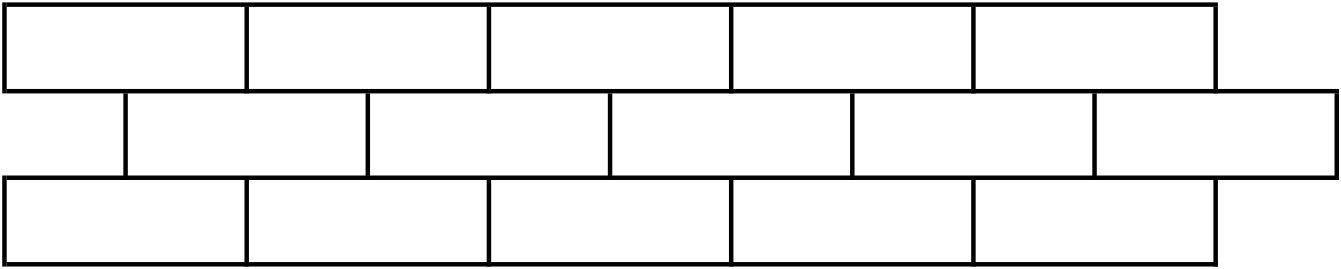
\includegraphics[width=8cm]{brick3x5}
	\end{figure}
	(b) Đếm số cách chọn ra 4 viên gạch, mỗi viên từ 1 hàng trong $4\times5$ viên gạch xếp xen kẽ, sao cho không có 2 viên gạch nào được lấy ra nằm kề nhau.
	\begin{figure}[H]
		\centering
		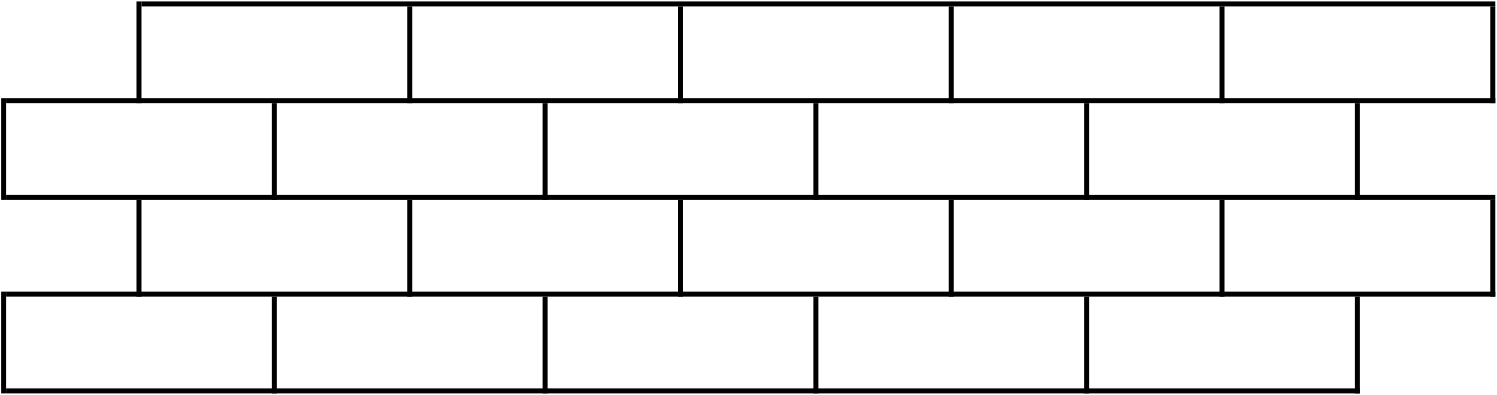
\includegraphics[width=8cm]{brick4x5}
	\end{figure}
	(c) Cho $m,n\in\mathbb{N}^\star$. Đếm số cách chọn ra $m$ viên gạch, mỗi viên từ 1 hàng trong $m\times n$ viên gạch xếp xen kẽ, sao cho không có 2 viên gạch nào được lấy ra nằm kề nhau. (d) Cho $m,n,k\in\mathbb{N}^\star$. Đếm số cách chọn ra $k$ viên gạch, không nhất thiết mỗi viên từ 1 hàng trong $m\times n$ viên gạch xếp xen kẽ, sao cho không có 2 viên gạch nào được lấy ra nằm kề nhau. (e${}^\star$) Mở rộng cho trường hợp $m\times n$ với số gạch mỗi hàng có thể khác nhau, cụ thể là hàng $i$ chứa $a_i\in\mathbb{N}^\star$ viên gạch, $\forall i = 1,\ldots,m$ với 2 trường hợp: (i) Mỗi viên từ 1 hàng. (ii) Lấy $k\in\mathbb{N}^\star$ viên gạch, mỗi hàng có thể lấy nhiều viên.
\end{baitoan}

\begin{nhanxet}[Left-right symmetry -- Đối xứng trái phải]
	Nếu số viên gạch của mỗi hàng bằng nhau \& được sắp xen kẽ như (a) \& (b), thì thứ tự viên gạch đầu tiên từ bên trái của mỗi hàng lồi ra hay thụt vào không quan trọng, vì có thể lấy đối xứng gương trái--phải để chuyển đổi 2 trường hợp đó. Cũng chú ý đến tính đối xứng trên--dưới (top-bottom symmetry).
\end{nhanxet}

\begin{itemize}
	\item C++ codes:
\end{itemize}

%------------------------------------------------------------------------------%

\section{Miscellaneous}

\subsection{Contributors}

\begin{enumerate}
	\item {\sc Võ Ngọc Trâm Anh}: ?.
	\item {\sc Đặng Phúc An Khang}: C++ codes.
	\item {\sc Nguyễn Lê Anh Khoa}: C++ codes.
	\item {\sc Phan Vĩnh Tiến}: \url{https://github.com/vinhtienlovemath/PublicDocuments/tree/main/MathematicalOlympiad}.
\end{enumerate}

\subsection{Donate or Buy Me Coffee}
Donate (not donut) or buy me some coffee via NQBH's bank account information at \url{https://github.com/NQBH/publication/blob/master/bank/NQBH_bank_account_information}.

\subsection{See also}

\begin{enumerate}
	\item {\it Olympic Tin Học Sinh Viên [OLP] \& ICPC}.
	
	PDF: {\sc url}: \url{https://github.com/NQBH/advanced_STEM_beyond/blob/main/OLP_ICPC/NQBH_OLP_ICPC.pdf}.
	
	\TeX: {\sc url}: \url{https://github.com/NQBH/advanced_STEM_beyond/blob/main/OLP_ICPC/NQBH_OLP_ICPC.tex}.
	\begin{itemize}
		\item Codes:
		\begin{itemize}
			\item C: \url{https://github.com/NQBH/advanced_STEM_beyond/tree/main/OLP_ICPC/C}.
			\item C++: \url{https://github.com/NQBH/advanced_STEM_beyond/tree/main/OLP_ICPC/C++}.
			\item Python: \url{https://github.com/NQBH/advanced_STEM_beyond/tree/main/OLP_ICPC/Python}.
		\end{itemize}
	\end{itemize}
\end{enumerate}

%------------------------------------------------------------------------------%

\printbibliography[heading=bibintoc]
	
\end{document}